% BEGIN LICENSE BLOCK
% Version: CMPL 1.1
%
% The contents of this file are subject to the Cisco-style Mozilla Public
% License Version 1.1 (the "License"); you may not use this file except
% in compliance with the License.  You may obtain a copy of the License
% at www.eclipse-clp.org/license.
% 
% Software distributed under the License is distributed on an "AS IS"
% basis, WITHOUT WARRANTY OF ANY KIND, either express or implied.  See
% the License for the specific language governing rights and limitations
% under the License. 
% 
% The Original Code is  The ECLiPSe Constraint Logic Programming System. 
% The Initial Developer of the Original Code is  Cisco Systems, Inc. 
% Portions created by the Initial Developer are
% Copyright (C) 2006 Cisco Systems, Inc.  All Rights Reserved.
% 
% Contributor(s): 
% 
% END LICENSE BLOCK

\chapter{A Tutorial Tour of Debugging in {\tkeclipse}}
\label{chapdebug}
%HEVEA\cutdef[1]{section}
 

This chapter demonstrates a sample debugging session using
{\tkeclipse}, showing how some of the 
development tools can be used. We are by no means using all the tools  or
all the functionalities of any tool, but hopefully this will give you a
flavor of the tools so that you will explore them on your own. You can get
more information on the tools from the \menu{Help} menu, and from the popup
balloons which appear when your mouse cursor stops over a feature for
a few seconds. 

In the tutorial tour, we will assume that you have some knowledge of
{\eclipse}. It is helpful if you also have some knowledge of
traditional Prolog debugging, although this is not necessary.

This chapter is designed for you to follow while running {\tkeclipse}.
To keep things simple, the program is run with a very small
data set, but it should be sufficient to see how the techniques described
can be applied to real programs. 

At the end of the chapter, there is a summary of the main features of the
main development tools.

This chapter
also contains many screen-shots, some of which are best viewed in colour, or
in looking at the actual screen as you follow along.

\quickref{Getting Help}{
\begin{description}
\item[Balloon help] A short description of a feature will popup in a
`balloon' when the mouse cursor stops over the feature for a few seconds.
\item[Help file] Help files are available for all the tools and
toplevel. They provide more detailed information on the tools, and can be
obtained from the \menu{Help} menu, and by typing Alt-h
(Alt and h keys together) in the tool.
\end{description}
}

\section{The Buggy Program}

The program we will be debugging is a map colouring problem. The 
task is to colour a
`map' of countries with four colours such that no two neighbours have the
same colour. Our program colours a map of four countries, but has a bug and
can colour two neighbours the same colour. The map is displayed graphically
as shown: 

\begin{center}
\parbox{0.43\textwidth}{\resizebox{0.4\textwidth}{!}{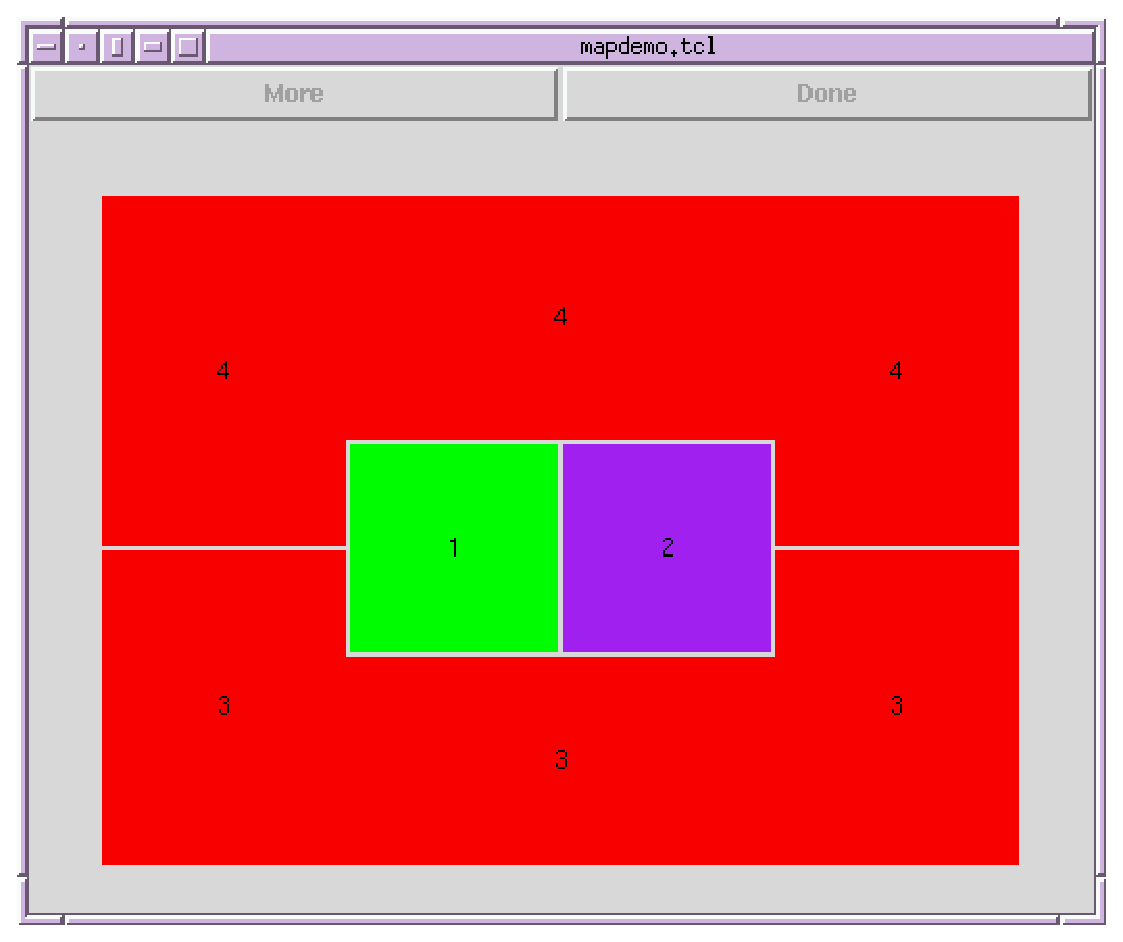
\includegraphics{mapdisplay2.ps}}}

\vspace{3mm}
{\bf Map Display of Program}
\end{center}

The countries are identified by numbers displayed within each country, and 
in this case, an incorrect colouring for the map is shown, because
countries 3 and 4 have the same colour. 

This program uses code from the map colouring demo program, and is
designed to use the GUI to display a map. Most of this is
not relevant to our debugging session, and although we will see some of this
code during the debugging, it is not necessary to understand it. 
You can think of this
debugging session as debugging someone else's code, not all of which
needs to be understood.

The program used here is included with your {\eclipse} distribution. You
should find it under the \texttt{doc/examples/tutorial} directory. You can
change to the \texttt{examples} directory in {\tkeclipse} using the
\menuopt{Change to example directory} option from the \menu{File} menu.

The final step in this debug tutorial is to edit the buggy program and
correct it. If you want to do this, you should copy the distributed version
of the program elsewhere so that you don't edit the original. You need to
copy the following files from \verb'examples/tutorial' to another directory:

\begin{quote}\begin{verbatim}
debugdemo.ecl  mapcolour.ecl mapdebugdemo.tcl buggy_data.map
\end{verbatim}\end{quote}

To load the program, start {\tkeclipse}. After start up, 
switch the working directory to
where you have the programs -- if you are using a UNIX system, and have
started {\tkeclipse} in the directory of the programs, you are already
there. Otherwise, go to the \menu{File} menu of {\tkeclipse}, and select
the \menuopt{Change directory} option. Use the directory browser to find
the directory containing your programs and select it. This will change your
working directory to the selected directory.

Next, compile \verb'debugdemo.ecl'. You can do this by selecting the
\menuopt{Compile} option from the \menu{File} menu (you can also compile
the file with the query \verb'[debugdemo]' from the query entry
window). 

\section{Running the Program}
To start the program, the query `colour' is run: type \verb'colour' 
into {\tkeclipse}'s query entry window, followed by the
return key. The program should run, and display the map to be coloured in a
window, which is then coloured, arriving at the
incorrect solution as shown previously. The program uses
the standard `generate-and-test' method, so you will see colour flashing in
the countries as the program tries different colours for them.

The map display has two buttons: pressing \button{More} will cause the program to
find an alternate way of colouring the map. Pressing \button{Done} will end the
program and return control to {\eclipse}. You can press \button{More} to get more
solutions and see that the program returns more solutions that colour
countries 3 and 4 to the same colour (along with some that are correct).

Press \button{Done} to finish the execution. We will now debug this program.

\section{Debugging the Program}


The main tool to debug a program is the {\bf tracer} tool. The tracer is
one of the development tools, all of which can be accessed from the \menuopt{Tools} menu of
{\tkeclipse}. Select \menuopt{Tracer} from the
menu as shown below, and a new window for the tracer tool should appear.

\begin{center}
\resizebox{0.5\textwidth}{!}{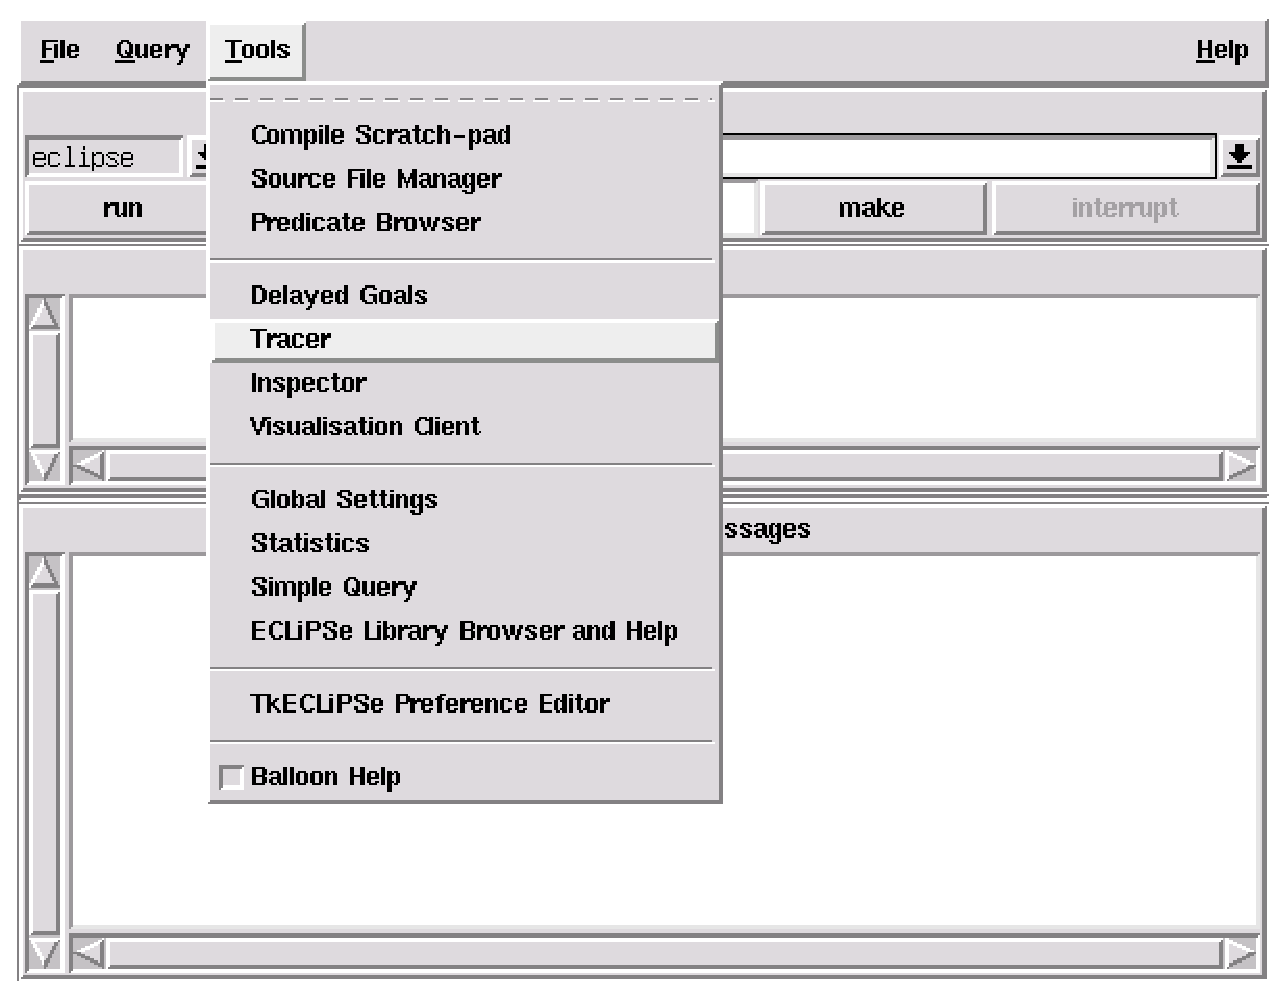
\includegraphics{tktoolsmenu.ps}}

\vspace{3mm}
{\bf Starting the Tracer Tool}
\end{center}
Run the query \verb'colour' again. To save you from typing in the query,
you can use the up-arrow on your keyboard to step back to a previous query.
Type return when  \verb'colour' appears in the query window again.

\begin{latexonly}
\begin{figure}
\begin{center}
\resizebox{0.35\textwidth}{!}{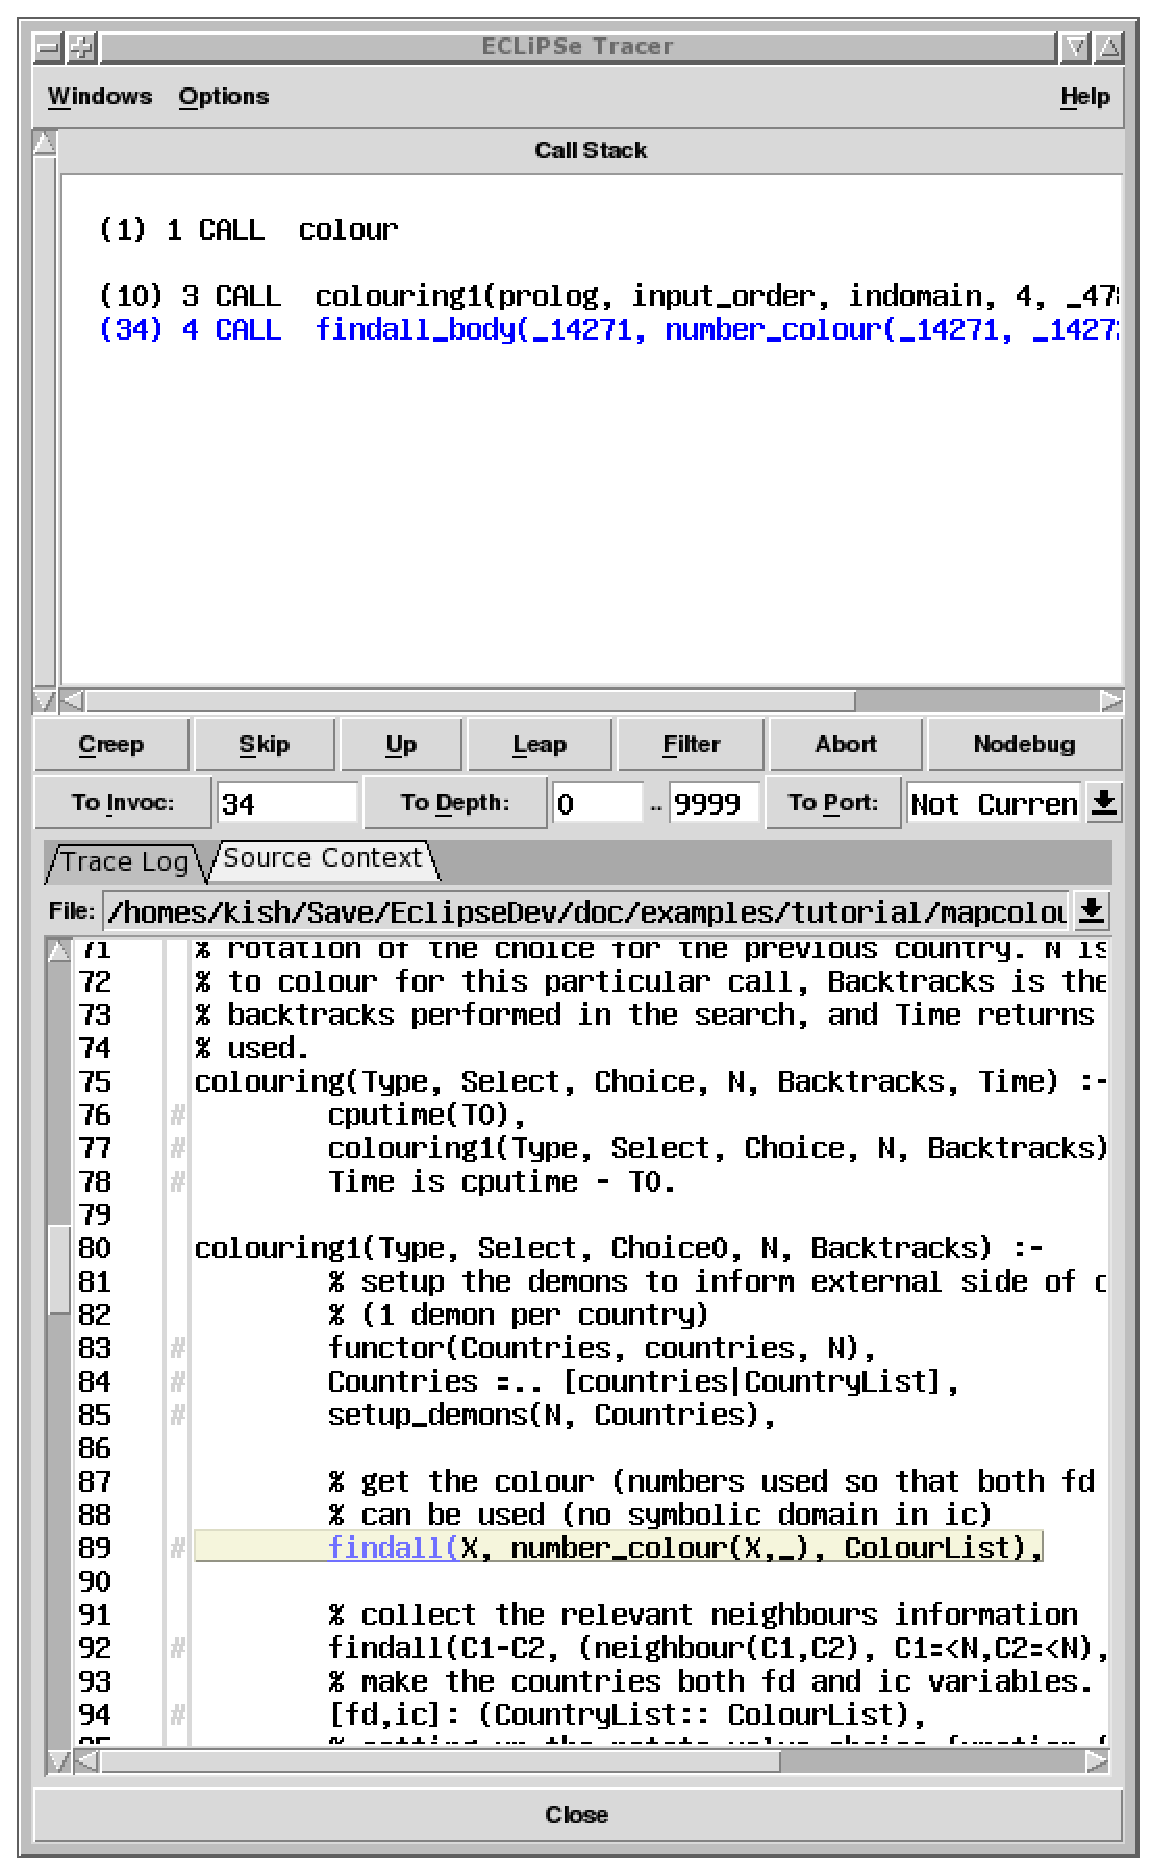
\includegraphics{tktracer.ps}}
\end{center}
\caption{The Tracer Tool}
\label{tktracer}
\end{figure}
\end{latexonly}

\begin{htmlonly}
\begin{figure}
\begin{center}
\resizebox{0.53\textwidth}{!}{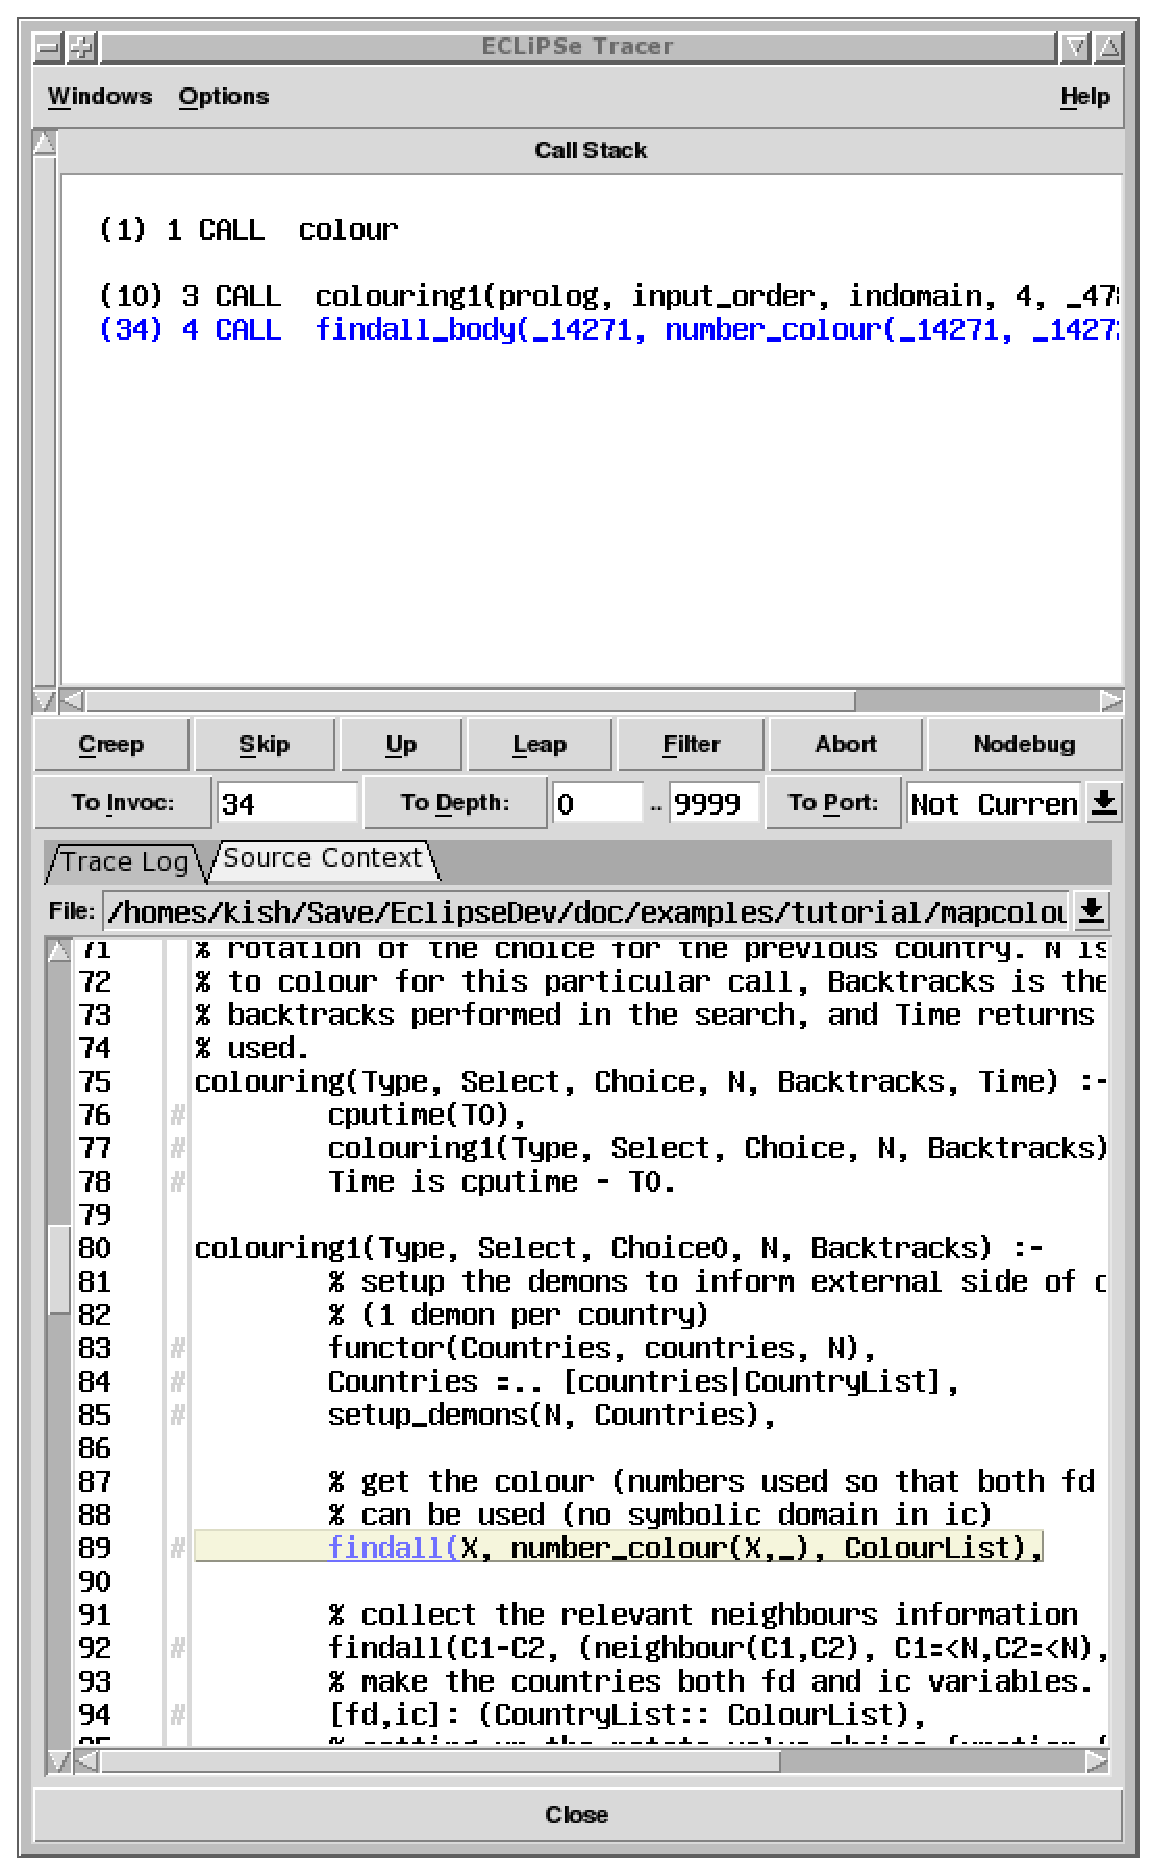
\includegraphics{tktracer.ps}}
\end{center}
\caption{The Tracer Tool}
\label{tktracer}
\end{figure}
\end{htmlonly}
\index{tracing program execution}
\index{tracer, development tool}

\quickref{Debugger Trace Line}{
\begin{small}
The trace lines displayed by the tracer has the following:
\begin{code}

 +(22) 14 *EXIT<3>  inform_colour(1, 1)

 1\quad2\quad\enspace3 4\quad\enspace5 6\qquad\qquad7

\end{code}
\begin{enumerate}
\item A '+' displayed here shows that the procedure has a spy point
  set. For a CALL port, a '\#' could be displayed in this position, which
  shows a breakpoint is set for the call.
\item The invocation number of this goal, which uniquely
  identifies it. The `To Invoc:' button can be used to jump to the next port with
  the specified invocation number. 
\item The depth of the goal, i.e. the number of its ancestors.
The `To Depth:' button can be used to jump to the next port within the specified
depth range.
\item An asterisk before an EXIT means that this
procedure is nondeterministic and that it might be resatisfied.
\item The type of the port. The `To Port:' button can be used to
  select the type of port to jump to.
\item This only appears if the goal is executing at a different priority
  than 12, the normal priority. The number is
  the priority that the  goal is executed at. 
\item The goal is printed according to the current instantiations
of its variables.  
\end{enumerate}
\end{small}
}

The tracer tool traces the execution of the program, like the traditional
Prolog debugger, it stops at  `debug ports' of predicates that are
executed.
\See{See the Debugging chapter in the User Manual for more details on the
  model used in Prolog debuggers.}
At the start of tracing,
it is stopped at the call port of the query \verb'colour'. The buttons in
the middle of the tool are for debugger commands. Try pressing
\button{Creep} several times, and you should observe something similar to
Figure~\ref{tktracer}. Unlike the traditional debugger, the execution trace
is shown on two text windows: the bottom `Source Context' view, showing the
execution of the program in the context of the source, highlighting the
body goal that corresponds to the goal at the debug port; and the
top `Call Stack' window, showing the ancestors (`call stack') of the
current goal, which is updated at each debug port. The goals are
displayed with different colours: blue for a call port, green (success) for
an exit port. Red (failure) for a fail port. Note that in the call
stack, the ancestor goals are displayed in black: this indicates that the
goal is not `current', i.e.\ the bindings shown are as they were when the
goal was called, and not necessarily what they are now. We will show how
these bindings can be `refreshed' later on. Note that the bottom windowc
can ne switched between the source context view, and a more traditional
`Trace Log' view, which shows a log of the debugger ports much as a traditional Prolog debugger does.

To avoid stepping through the whole program, we will add a spy-point to a
predicate that may be causing the problem. Spy-points can be added in the
traditional way, using the \verb'spy/1' predicate. However, we can also use
the {\bf predicate browser} tool:  start the \menuopt{Predicate Browser} tool
from the \menu{Tools} menu of {\tkeclipse}. This tool allows you to observe
and change various properties of the predicates in your program.
A list of predicates are displayed
on the left hand side, and a list of properties on the right.
Currently the predicate list is showing all the predicates defined in our program (i.e.\ in
the \verb'eclipse' module). Looking at this list,
\verb'not_same_colour/3''s name suggests that
it checks that neighbouring countries do not have the same colour.
Select it by clicking on it, and now the right
hand side should display the properties of this predicate:

\begin{center}
\resizebox{0.55\textwidth}{!}{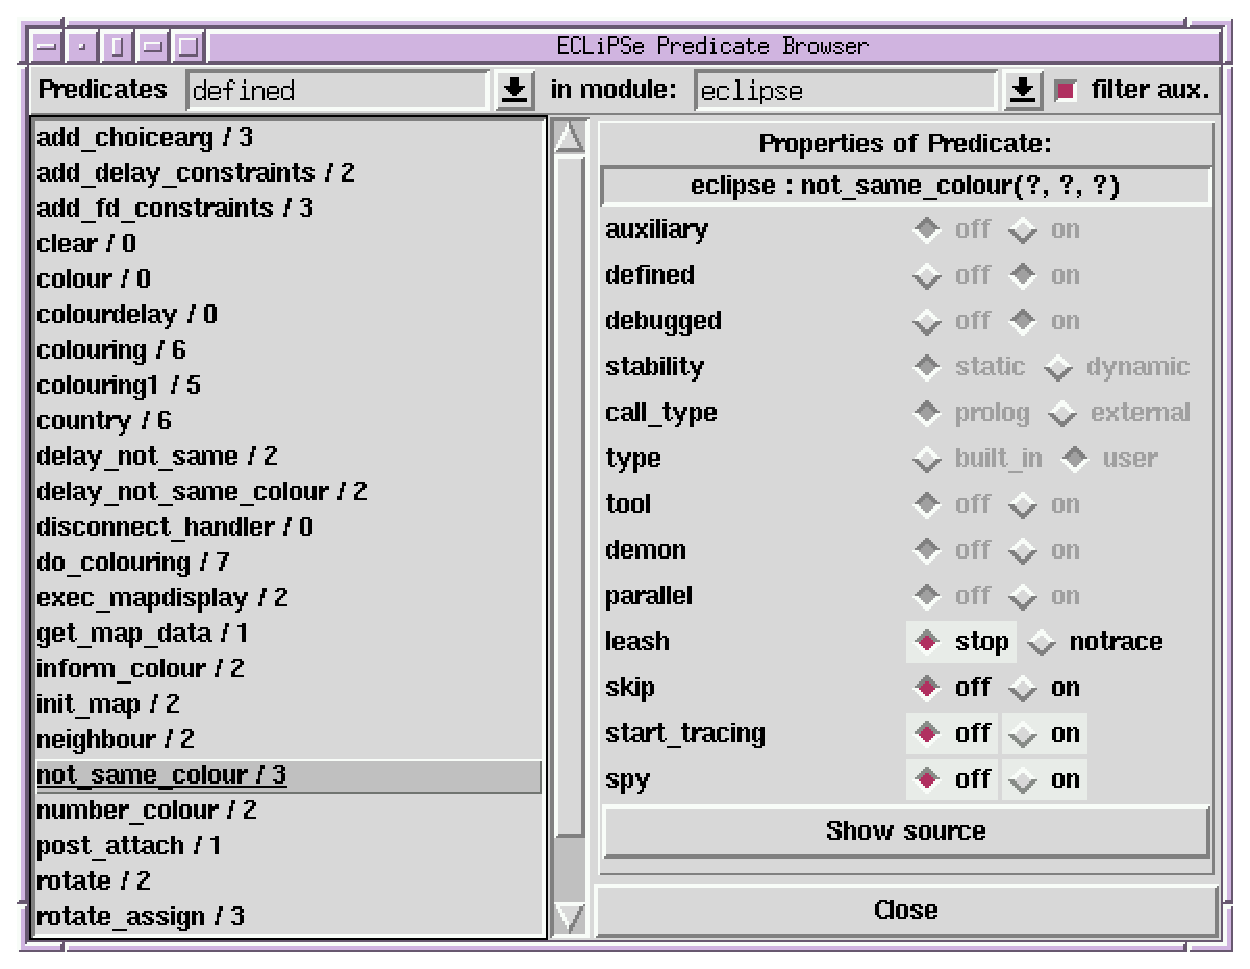
\includegraphics{tkpredbrowser.ps}}

\vspace{3mm}
{\bf The Predicate Browser Tool}
\end{center}
\index{predicate browser, development tool}

We can now view the source code for the predicate by clicking on the
\button{Show source} button, which will show the selected predicate's source in
the source context view. The code for the predicate is:

\begin{code}
not_same_colour(Solver, C1-C2, Countries) :-
      % get the colours for the countries C1 and C2
      arg(C1, Countries, Colour1),
      arg(C2, Countries, Colour2),
      % send constraint to either the fd or ic solver
      Solver: (Colour1 #\verb'\'= Colour2).
\end{code}

The code does indeed check that the countries \verb'C1' and \verb'C2' do
not have the same colour.

\Note{For our example program, the list is not very long, but some programs may
have many predicates, and it could be difficult to find the predicate you
want. The predicate list has a search facility: typing in part of the name
of the predicate in the predicate list will search for the predicate you
want. You can try typing in {\tt not_same_colour / 3} to see how this
works.}

The predicate browser allows us to change some of the properties of a predicate.
We can add a spy-point to the predicate by clicking on the radio button for
{\bf spy}: 

\begin{center}
\resizebox{0.27\textwidth}{!}{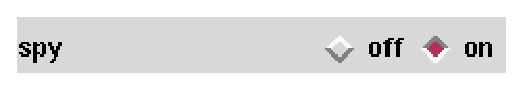
\includegraphics{tkpredspyon.ps}}

\vspace{2mm}
{\bf Setting Spy Property to On}
\end{center}

With {\tkeclipse}, we can do more than just place a spy point on a
predicate: we can specify further conditions for when the tracer should
stop at a spy point, using the filter tool. 

Start the filter tool by selecting \menuopt{Configure filter} from the \menu{Options} menu of the tracer
tool:

\begin{center}
\resizebox{0.4\textwidth}{!}{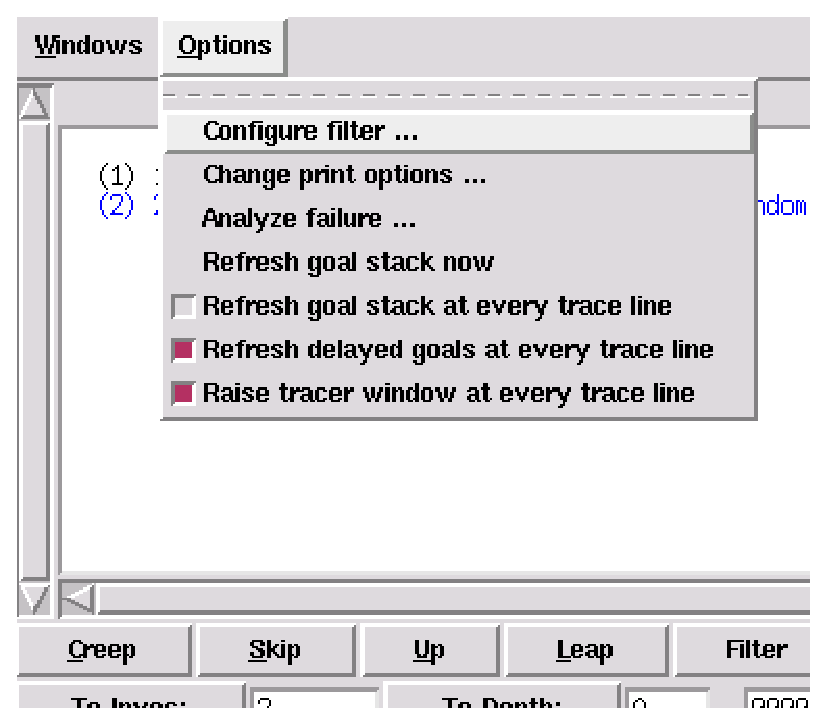
\includegraphics{tktraceroptions.ps}}

\vspace{3mm}
{\bf Starting the Filter Tool from the Tracer}
\end{center}

\begin{figure}
\begin{center}
\resizebox{0.5\textwidth}{!}{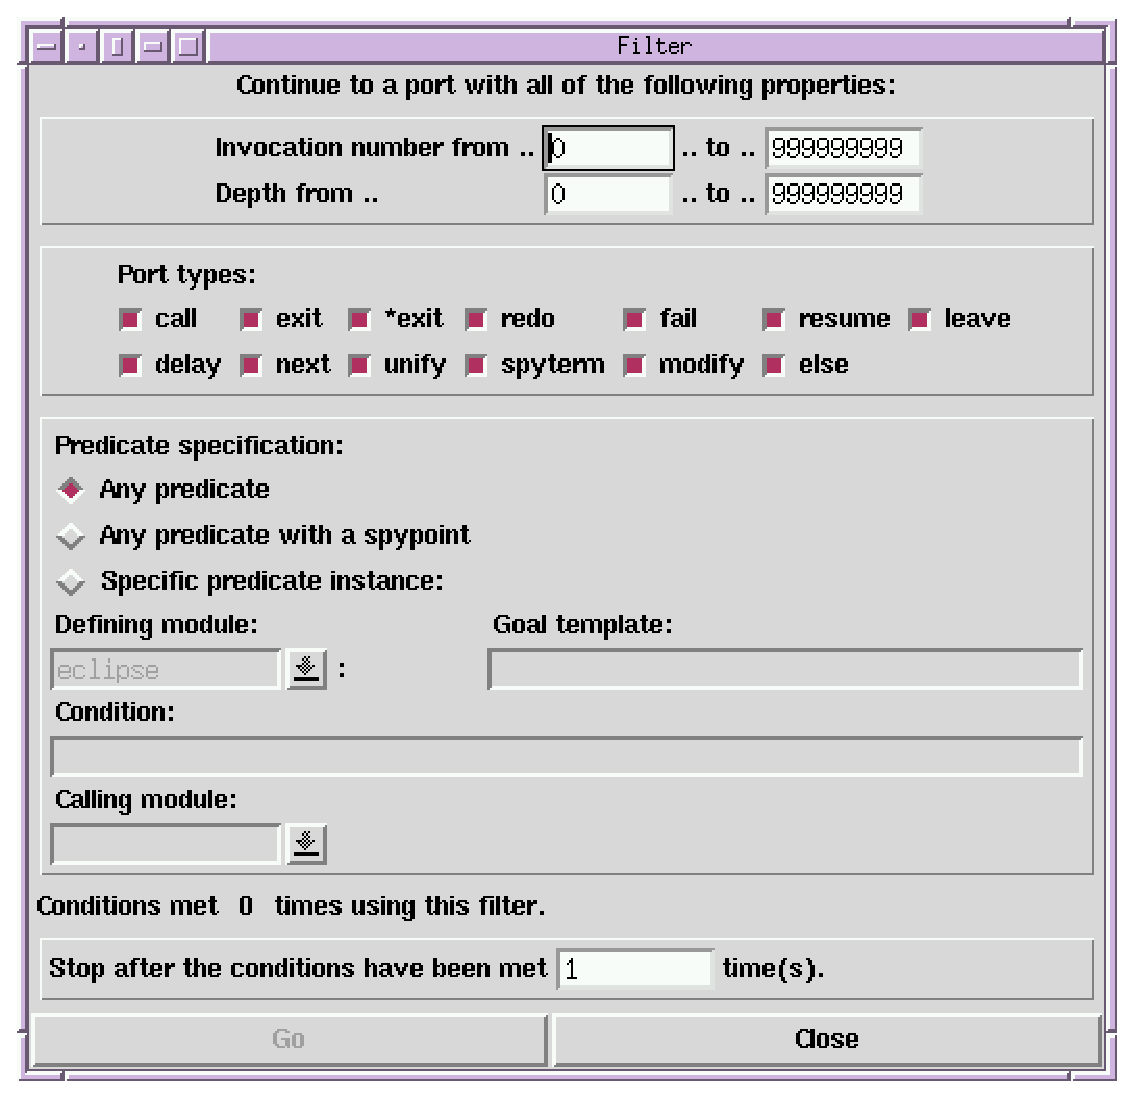
\includegraphics{tkfilter.ps}}
\end{center}
\caption{The Tracer Filter Tool}
\label{tkfilter}
\end{figure}

The filter tool opens in a new window, as shown in
Figure~\ref{tkfilter}. This tool allows us to specify a `filter' for the
debug ports so that the tracer will only stop at a port with the properties
specified by the tool. In our case, we want to see \verb'not_same_colour/3'
only when countries 3 and 4 are involved. This can be done 
with the ``Predicate specification'' facility, enabled by the
\button{Specific predicate instance:} radio button. Pressing this button
will allow us to specify a condition in Prolog syntax which will be
checked at each debug port. For our purpose, we enter the following:

\begin{center}
\resizebox{0.55\textwidth}{!}{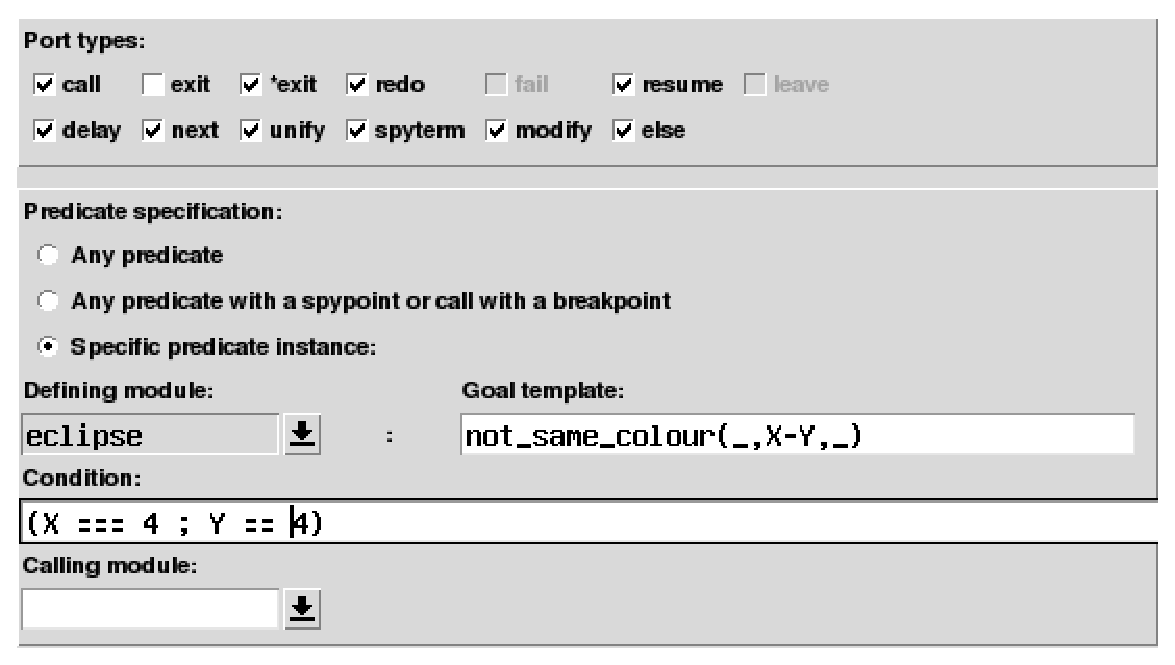
\includegraphics{tkfiltercond.ps}}

\vspace{3mm}
{\bf Setting Conditions for Specific Predicate Instances}
\end{center}

\index{conditional spying}
\index{tracer filter, development tool}
This specifies that the filter should stop at a \verb'not_same_colour/3'
goal, when one of the countries in the pair \verb'X-Y' is country 4: the {\bf
Goal template} is used to specify the template the debug port goal should
match, and the {\bf Condition:} can be any {\eclipse} goal, perhaps with variables
from the {\bf Goal template}, as in our case. The test is done by unifying
the goal with the template, and then executing the condition. Note that any
bindings are undone after the test. 

Note that we have also deselected the \button{exit} port in the filter
condition. You can do this by clicking on the \button{exit} radio
button. This means that the tracer does not stop at any exit port.

Press \button{Go} on the filter tool to start the tracer running with the
filter. You can also press the \button{Filter} command button on the tracer
to do the same thing.
We see that the tracer has jumped to a \verb'not_same_colour/3' goal
involving country 4 as expected. However, there is a gap in the call stack
as we skipped over the tracing of some ancestor goals. We can see these
goals by {\bf refreshing} the goal stack. This can be done by pressing and
holding down the right mouse button while the mouse cursor is over a goal
in the call stack, which will popup a menu for the goal:

\begin{center}
\resizebox{0.55\textwidth}{!}{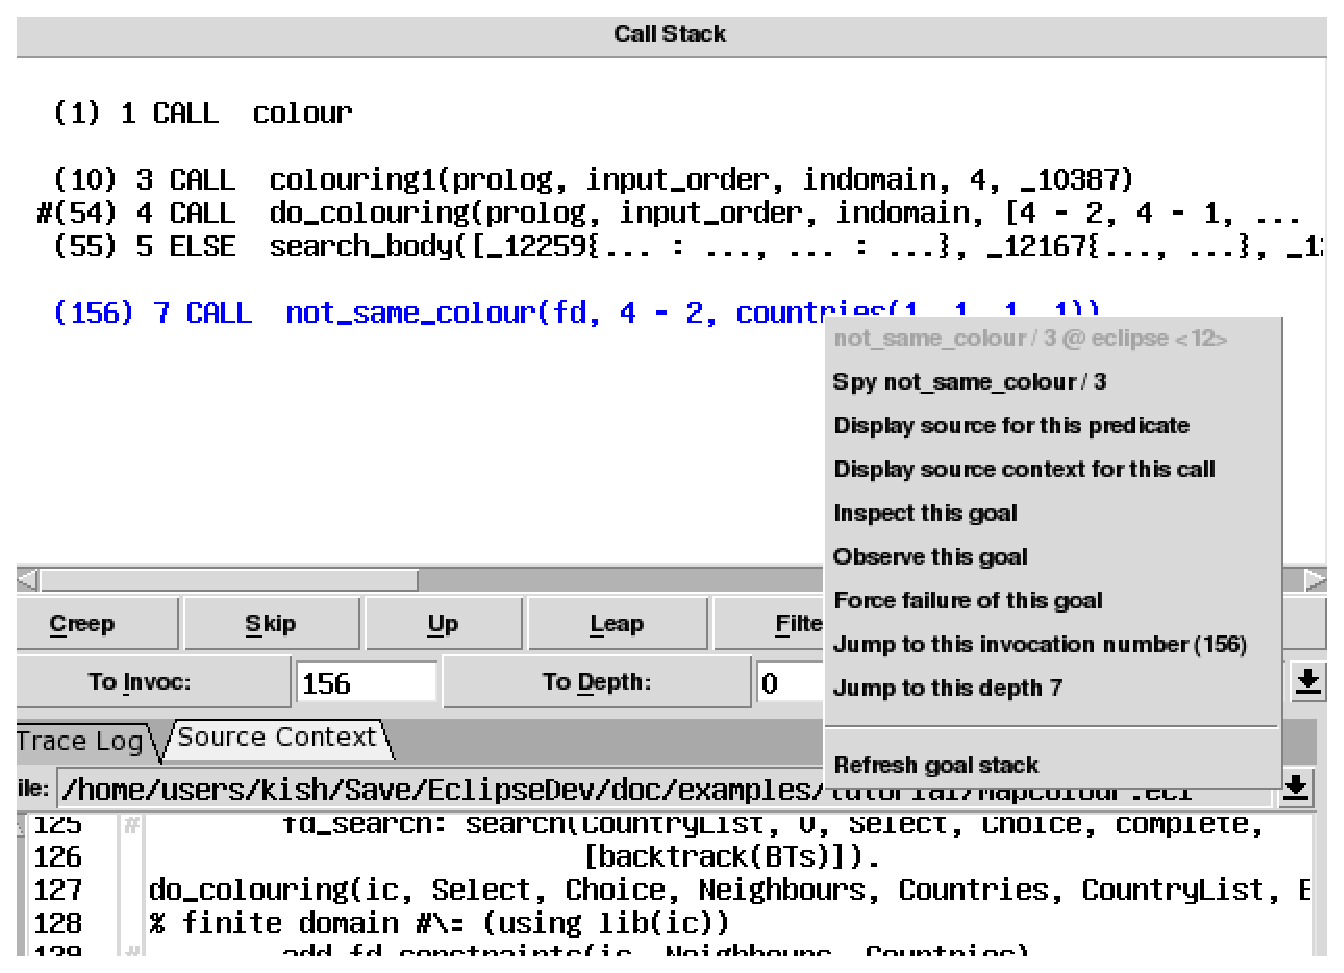
\includegraphics{tktracerpopup.ps}}

\vspace{3mm}
{\bf Popup Menu for a Goal in Tracer's Call Stack}
\end{center}

In this case, we have opened the menu over \verb'not_same_colour/3', and the
options are for this goal. Various options are available, but for now we
choose the \menuopt{Refresh goal stack} option. This will result in the
following goal stack display:

\begin{center}
\resizebox{0.6\textwidth}{!}{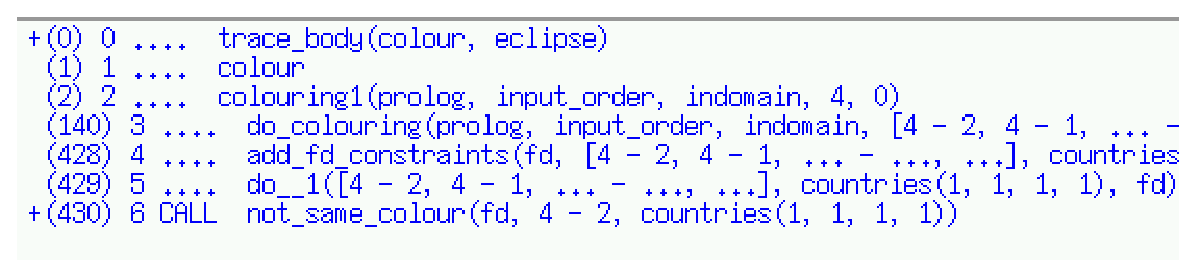
\includegraphics{tkrefreshedgs.ps}}

{\bf Refreshed Call Stack}
\end{center}

Notice that the colour of the goals in the goal stack are now all blue,
indicating that the bindings shown are current. 

Press \button{Filter} on the tracer several times to jump to other ports
involving country 4. You will see that none of them involve countries 3 and
4. So perhaps countries 3 and 4 are not checked by
\verb'not_same_colour/3', i.e.\ \verb'3-4' or \verb'4-3' are never passed
to \verb'not_same_colour/3'. Looking at the call stack, we can see that the
country pair in \verb'not_same_colour/3' seem to appear as an element in a
list of country pairs, as far back as \verb'colouring(...)'. Unfortunately,
the debugger does not display the whole list. We see something like:

\begin{center}
\verb'do_colouring(prolog, input_order, indomain, [4 - 2, 4 - 1, ... '
\end{center} 
\noindent
due to the `print depth' feature, which shortens the printing of large
terms. We can examine the whole list by using the inspector to examine the
goal. To do this, we double click on the \verb'do_colouring(...)' goal
to `open' it for inspection.

This will launch the Inspector tool on the \verb'do_colouring' goal. The
inspector displays the term in a hierarchical fashion as a tree, which
allows us to navigate the term. The initial display is shown on the left
panel below. We are interested in examining the full list. We can look at
this list by double clicking on it to expand the node, which results in the
display in the right panel below. You may need to scroll
down to see the whole list:

\begin{center}
\parbox{0.49\textwidth}{\resizebox{0.48\textwidth}{!}{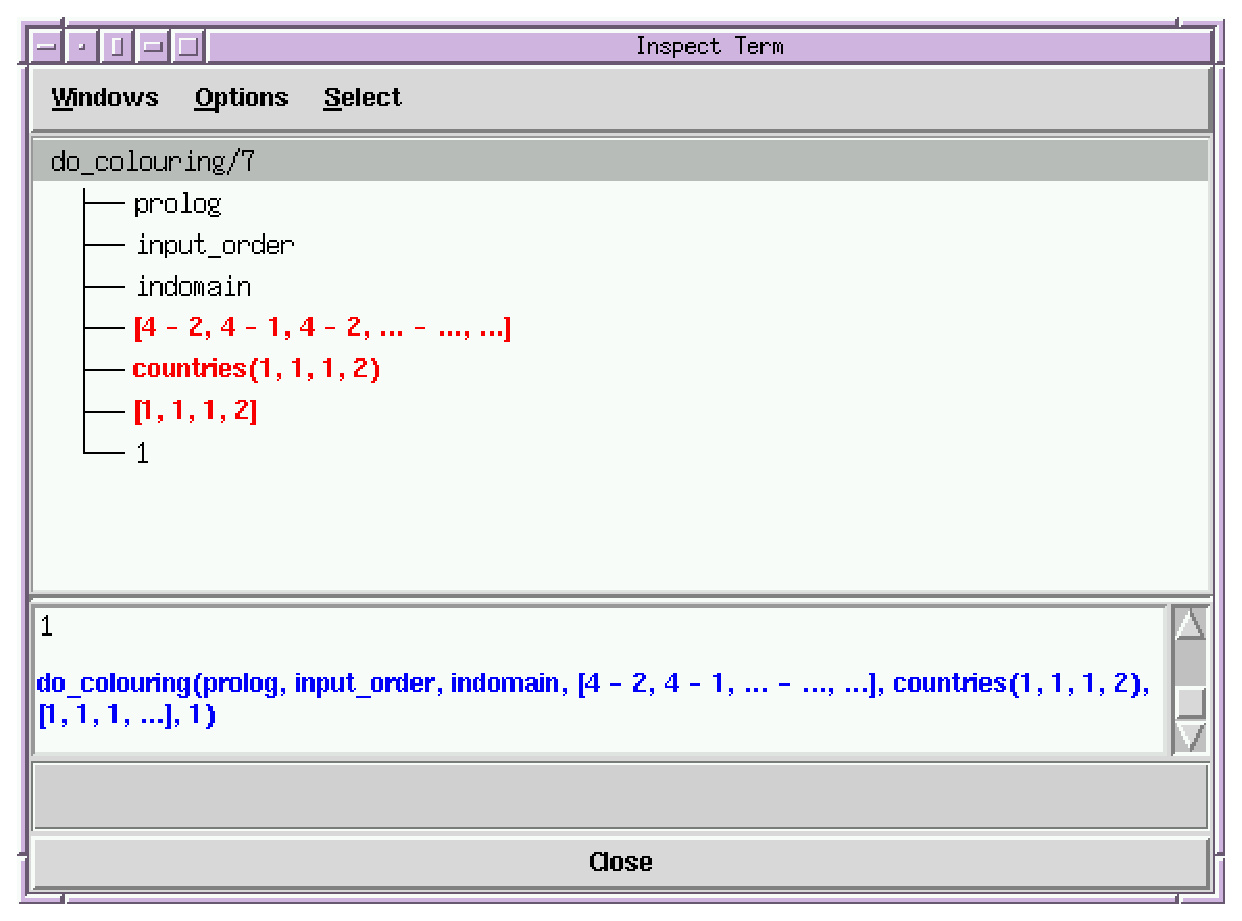
\includegraphics{tkinspect.ps}}}
\parbox{0.49\textwidth}{\resizebox{0.48\textwidth}{!}{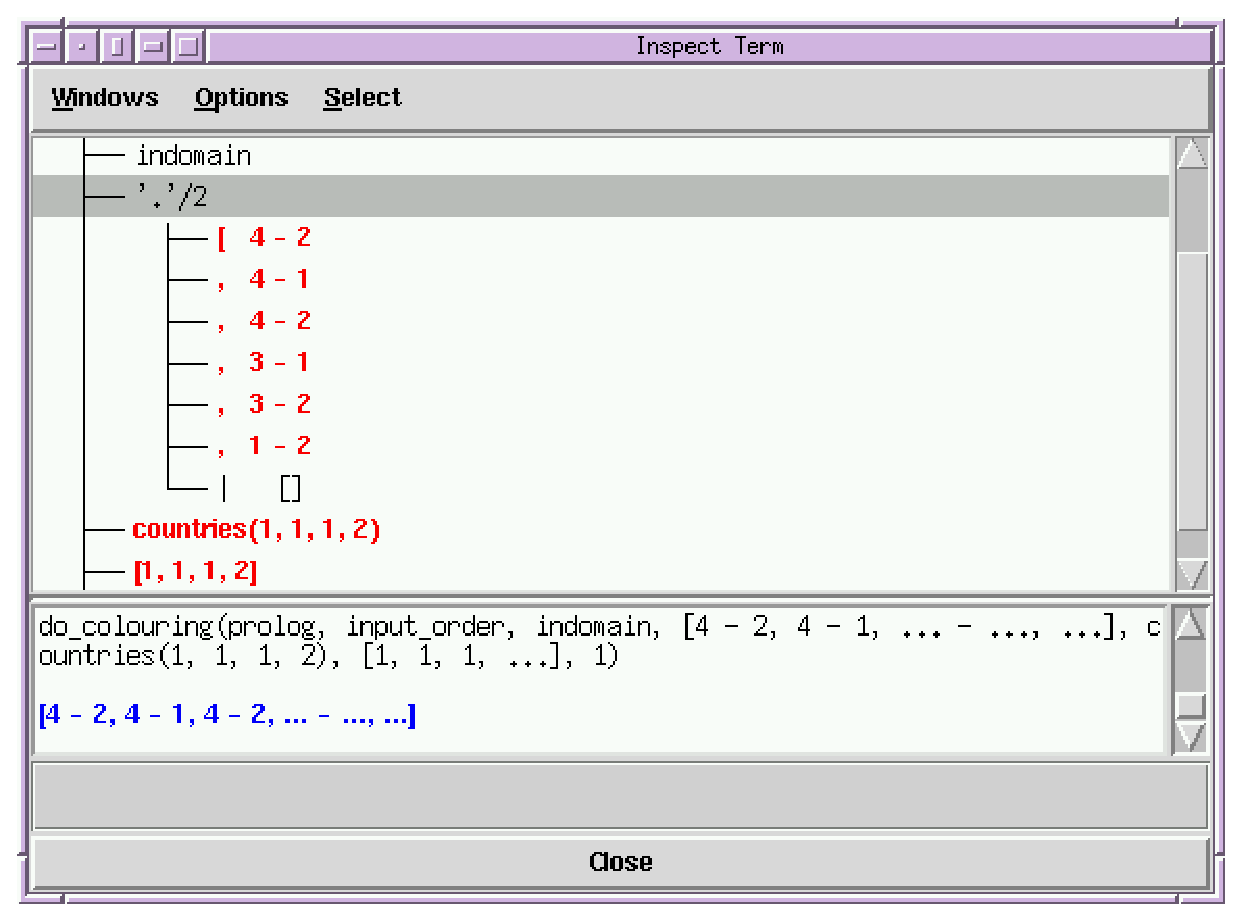
\includegraphics{tkinspect2.ps}}}

\vspace{3mm}
{\bf Using the Inspector}
\end{center}

\index{term inspector, development tool}
\index{inspecting terms}
The inspector shows that this list does not contain the pair \verb'4-3' or
\verb'3-4', which should be there so that \verb'not_same_colour'
can check that these two countries  are not assigned the same colour.

\begin{sloppypar}
The inspector tool is modal -- when it is open, the rest of {\tkeclipse} is
inaccessible. Close the Inspector by clicking on its
\button{Close} button, go back to the tracer, and see where the country
pair list comes from. It
first appears in 
the ancestor goals \verb'do_colouring(prolog,...)', as the next parent
\verb'colouring(prolog,...)' does not have this list. So the list
is created in a body goal of \verb'colouring(...)' before \verb'do_colouring(...)' is
called. We can look at the source of \verb'colouring(...)'  to see how this
list is created. To do this, we can
select \menuopt{Display source} option from the popup menu for the
\verb'colouring(...)' goal:
\end{sloppypar}
 
\begin{center}
\resizebox{0.55\textwidth}{!}{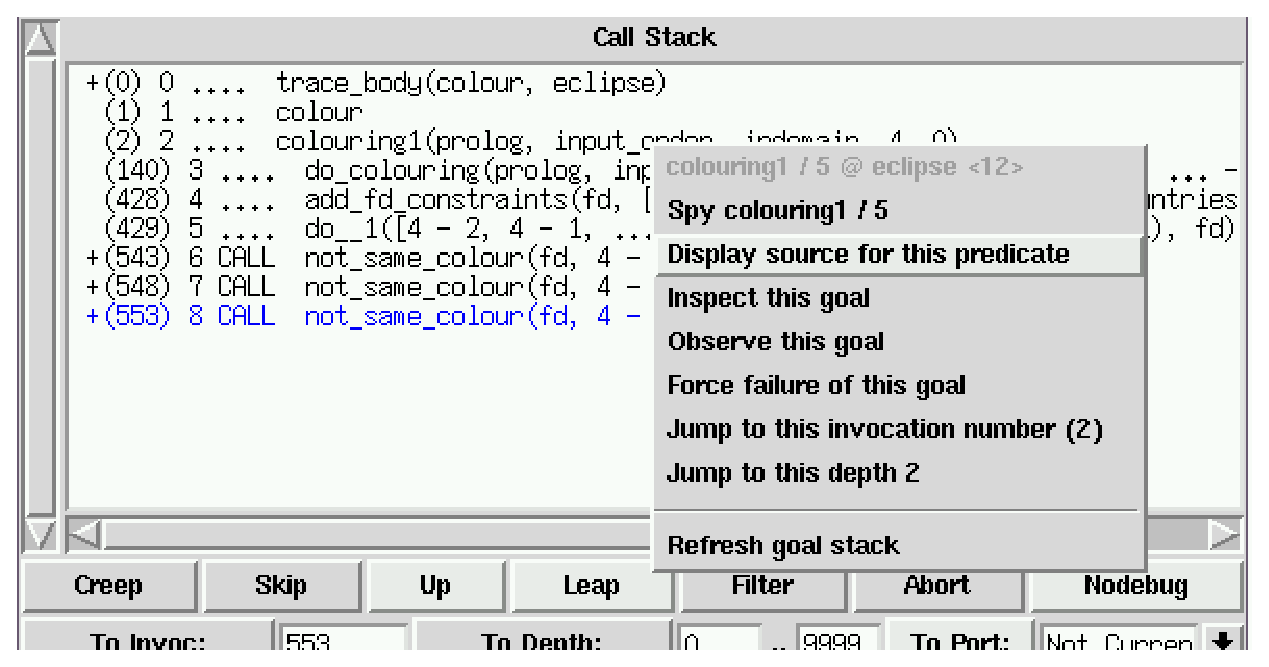
\includegraphics{tktracerpopup2.ps}}

\vspace{3mm}
{\bf Displaying Source for a Goal in the Call Stack}
\end{center}

The code for this predicate is quite long, but for our purposes we are only
interested in the country-pair list that is passed to \verb'do_colouring':

\begin{code}
colouring1(Type, Select, Choice0, N, Backtracks) :-
        ....
        findall(C1-C2, (neighbour(C1,C2), C1=<N,C2=<N), Neighbours),
        ....
        do_colouring(Type, Select, Choice, Neighbours, Countries,
                     CountryList, Backtracks), 
        ....
\end{code}

Looking at this source and the Call stack goal, we can see that the country
pair list is constructed from \verb'neighbour/2' calls. Let's look at the
source for \verb'neighbour/2'. We can do this from the predicate browser, by
selecting \verb'neighbour/2' and pushing the \button{Show source} button. We see
the following:

\begin{code}
neighbour / 2 in file buggy_data.map, line 2:
%neighbour(4, 3).
neighbour(4, 2).
neighbour(4, 1).
neighbour(4, 2).
neighbour(3, 1).
neighbour(3, 2).
neighbour(1, 2).
\end{code}


So \verb'neighbour(4,3)' was indeed missing (it is commented out).
Another way to check \verb'neighbour/2', without looking at the source,
would be using the
Simple Query tool. This tool is again started from {\tkeclipse}'s
\menu{Tools} menu. It can be used to send simple queries to {\eclipse},
even while another query is being executed (as we are here, executing the
\verb'colour' query). We can use this tool to check if \verb'neighbour(4,3)'
or \verb'neighbour(3,4)' are defined or not:

\begin{center}
\resizebox{0.55\textwidth}{!}{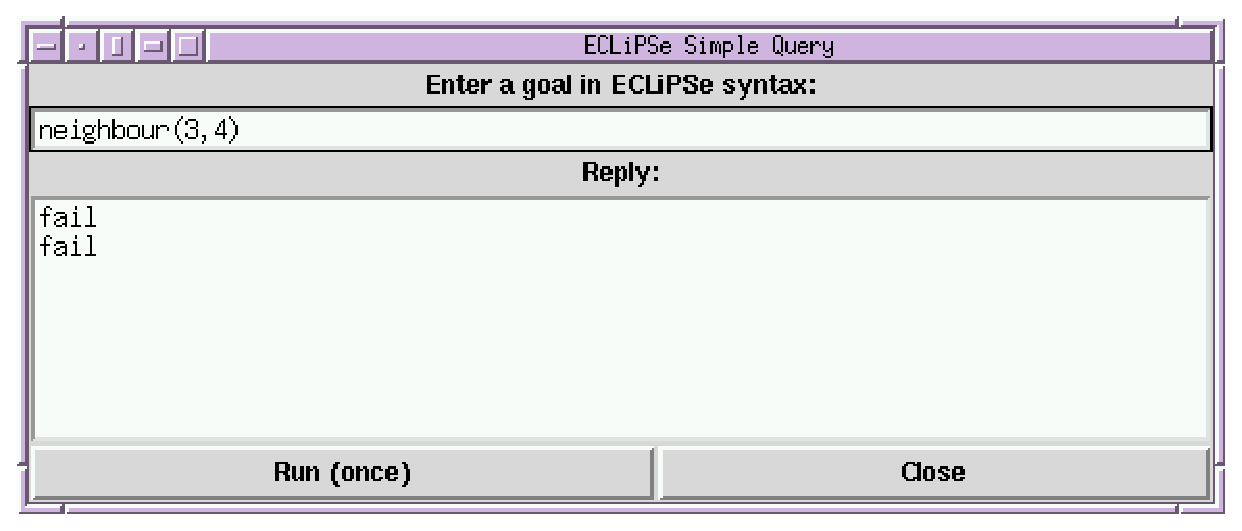
\includegraphics{tkquery.ps}}

\vspace{3mm}
{\bf The Simple Query Tool}
\end{center}

To send a query, simply type it in the entry window and press return, and
the reply will be sent to the reply window. In the example above, we have
tried \verb'neighbour(4,3)', followed by \verb'neighbour(3,4)', and
both failed, indicating that there is no neighbour relationship defined
between countries 3 and 4.

\begin{sloppypar}
 We can fix the program by editing
the file \verb'buggy_data.map' and adding the neighbour(4, 3) line back.
TkECLiPSe does not provide an integrated editor itself, so you need to use
some external editor, such as emacs, vi, or wordpad to edit the program. 
You can tell \eclipse which editor you want to use, so that you can invoke
the editor from within \eclipse. For example, from the source context view
window of the tracer, you can invoke an editor to edit the file being
\begin{figure}
\begin{center}
\resizebox{0.3\textwidth}{!}{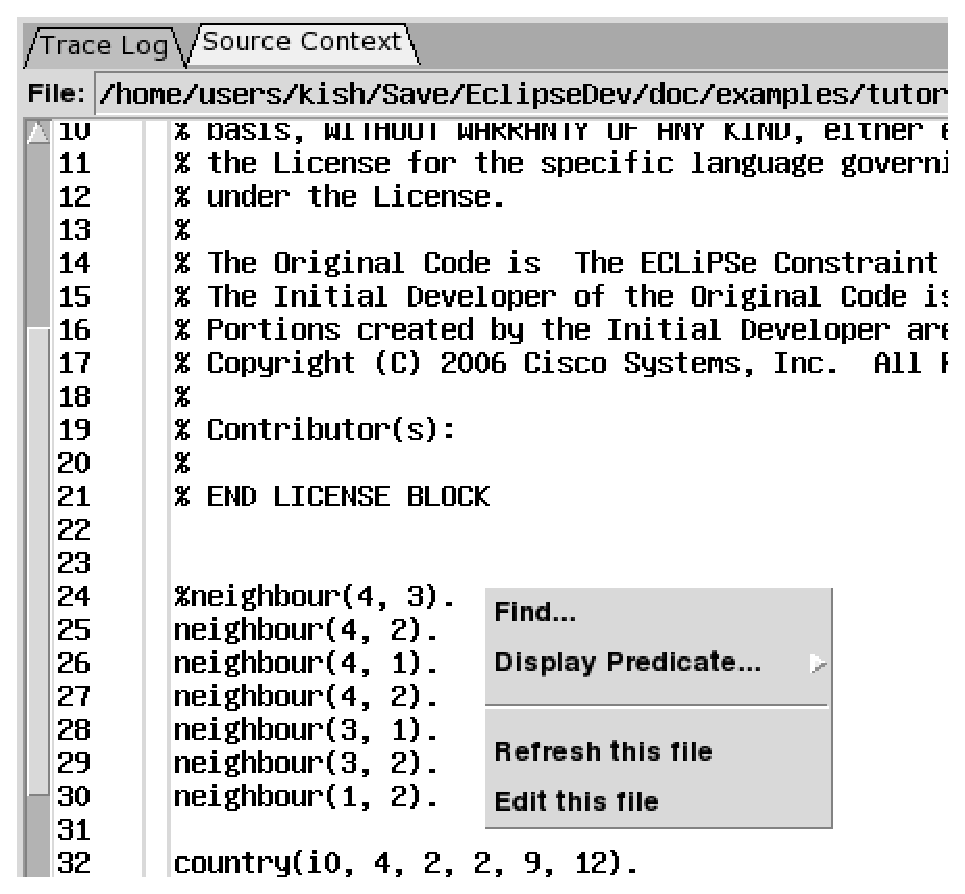
\includegraphics{tksoucontext.ps}}
\end{center}
\caption{Invoking an editor}
\label{tkeditor}
\end{figure}
displayed. Holding down your right mouse button in the source context
window will popup a menu, as shown in figure~\ref{tkeditor}. Select ``Edit
this file'' option will invoke your specified editor to edit the file, and if
possible, the file will be opened showing the line where your mouse pointer
was when you popup the menu (line 24 in this example).

\Note{
You can specify an editor to use with \eclipse using the Tkpreference
editor tool from the Tools menu. Fill in the entry for ``Text editor to use''
with the editor you want to use -- this should be the command that you will
type in a command line to invoke your editor. In addition, if your editor
supports it, you can fill in
the ``Editor's command line option to start at a specific line'' with the
command line option that will cause the editor to open the file at a
certain line.
}

To run the corrected program, we first end our current debugging session by
closing the tracer window. You can see from the map display that the
execution continues until a solution is produced. 
Pressing \button{Done} on the map display will return control to
{\eclipse}. Alternatively, if continuing the execution is undesirable,  press the \button{Abort} command button in
the tracer, which would abort the execution.
\end{sloppypar}

Once we have made the correction to the program and saved it,
we compile it by pressing the
\button{Make} button on {\tkeclipse}. This recompiles any files that
have been updated since {\eclipse} last compiled the file. 

Running the program again will show that the bug is indeed fixed.


\quickref{Mouse Button Operations on Objects}{
In {\tkeclipse}, you can usually perform these operations on an object
while the mouse cursor is over it:

\begin{description}
\item[left-click] selects the object. 
\item[double (left)-click] `opens' the object. This can mean expanding it
(e.g. in the inspector), or calling the inspector on it (e.g.\ on a goal in
the call stack), or showing the source for a goal (e.g. in the source
context view).
\item[Right-click and hold]  Opens a menu which gives
further option/information on the object.
\end{description}
Right-mouse button functionality are alternatively available through the
left-mouse button with the control key pressed.
}

\quickref{Available Development tools}{
{\small
\begin{description}
\item[Compile scratch pad] allow simple programs to be written and
compiled. Equivalent to {\tt [user]} in command line {\eclipse}.
\item[Source file manager] manage source files for this {\eclipse} session.
\item[Predicate browser]  view/change properties of predicates.
\item[Delayed goals] view delayed goals.
\item[Tracer] debugger for {\eclipse} programs.
\item[Inspector] term inspector. Useful for viewing large terms.
\item[Visualisation client] start a visualisation client.
\item[Global settings] view/change global {\eclipse} settings.
\item[Statistics] show statistics. Information is updated dynamically.
\item[Simple query] send simple queries to {\eclipse}.
\item[Library browser and help] interface to {\eclipse} documentation.
\item[TkECLiPSe preference editor] view/change {\tkeclipse} settings. 
\end{description}
}}

\section{Summary}
\subsection{{\tkeclipse} toplevel}
\index{toplevel}
\resizebox{0.8\textwidth}{!}{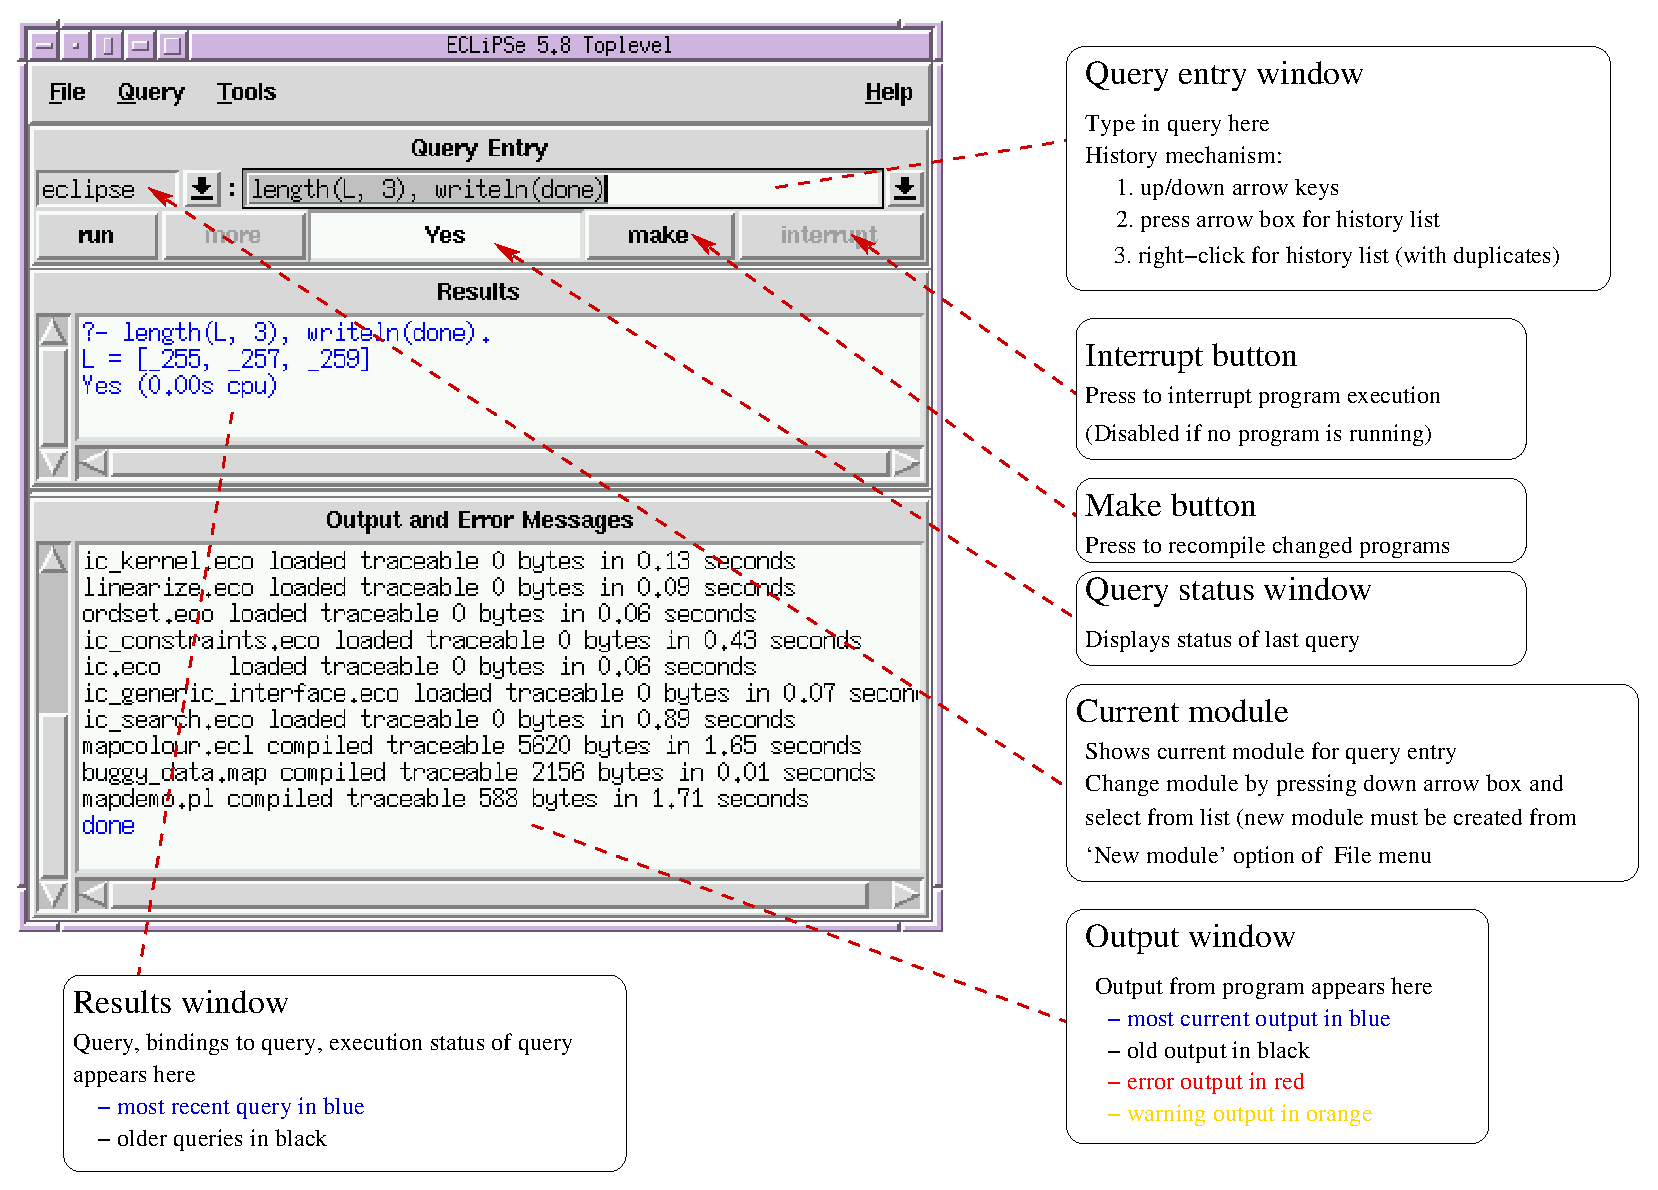
\includegraphics{tktopann.eps}}

\subsection{Predicate Browser} 
\index{predicate browser, development tool}
\resizebox{0.8\textwidth}{!}{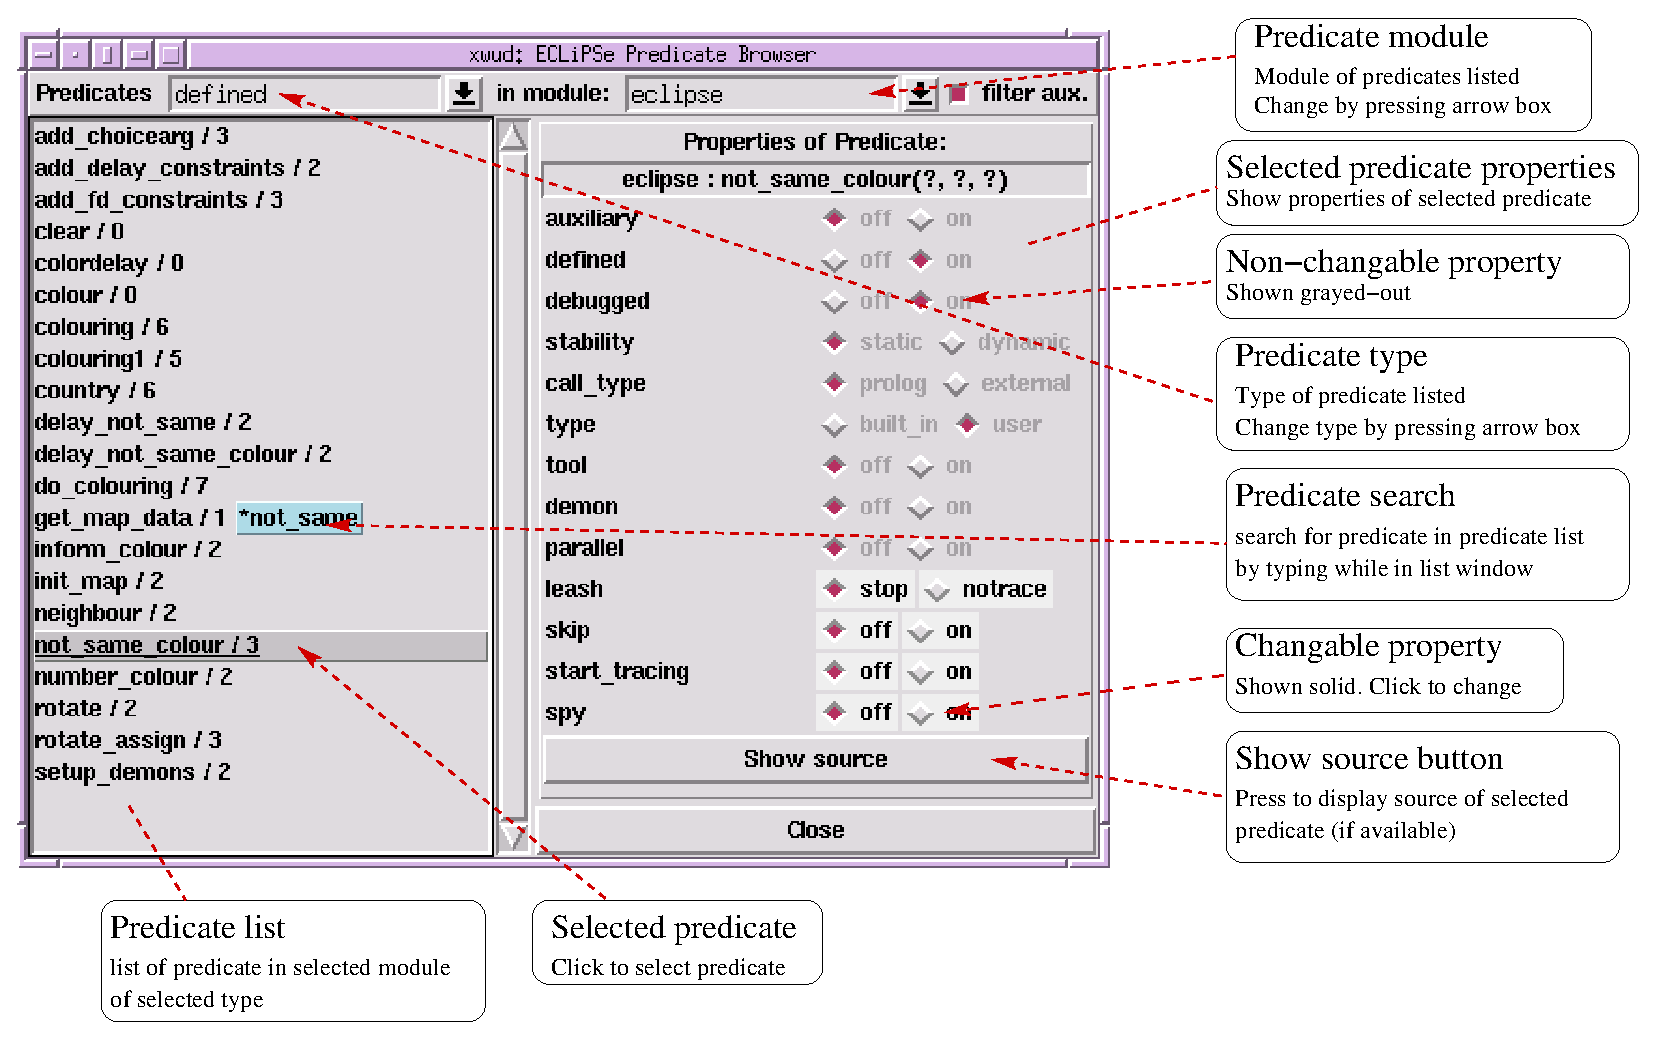
\includegraphics{tkpredann.eps}}

\subsection{Delayed Goals Viewer}
\index{delayed goals viewer, development tool}

\resizebox{0.7\textwidth}{!}{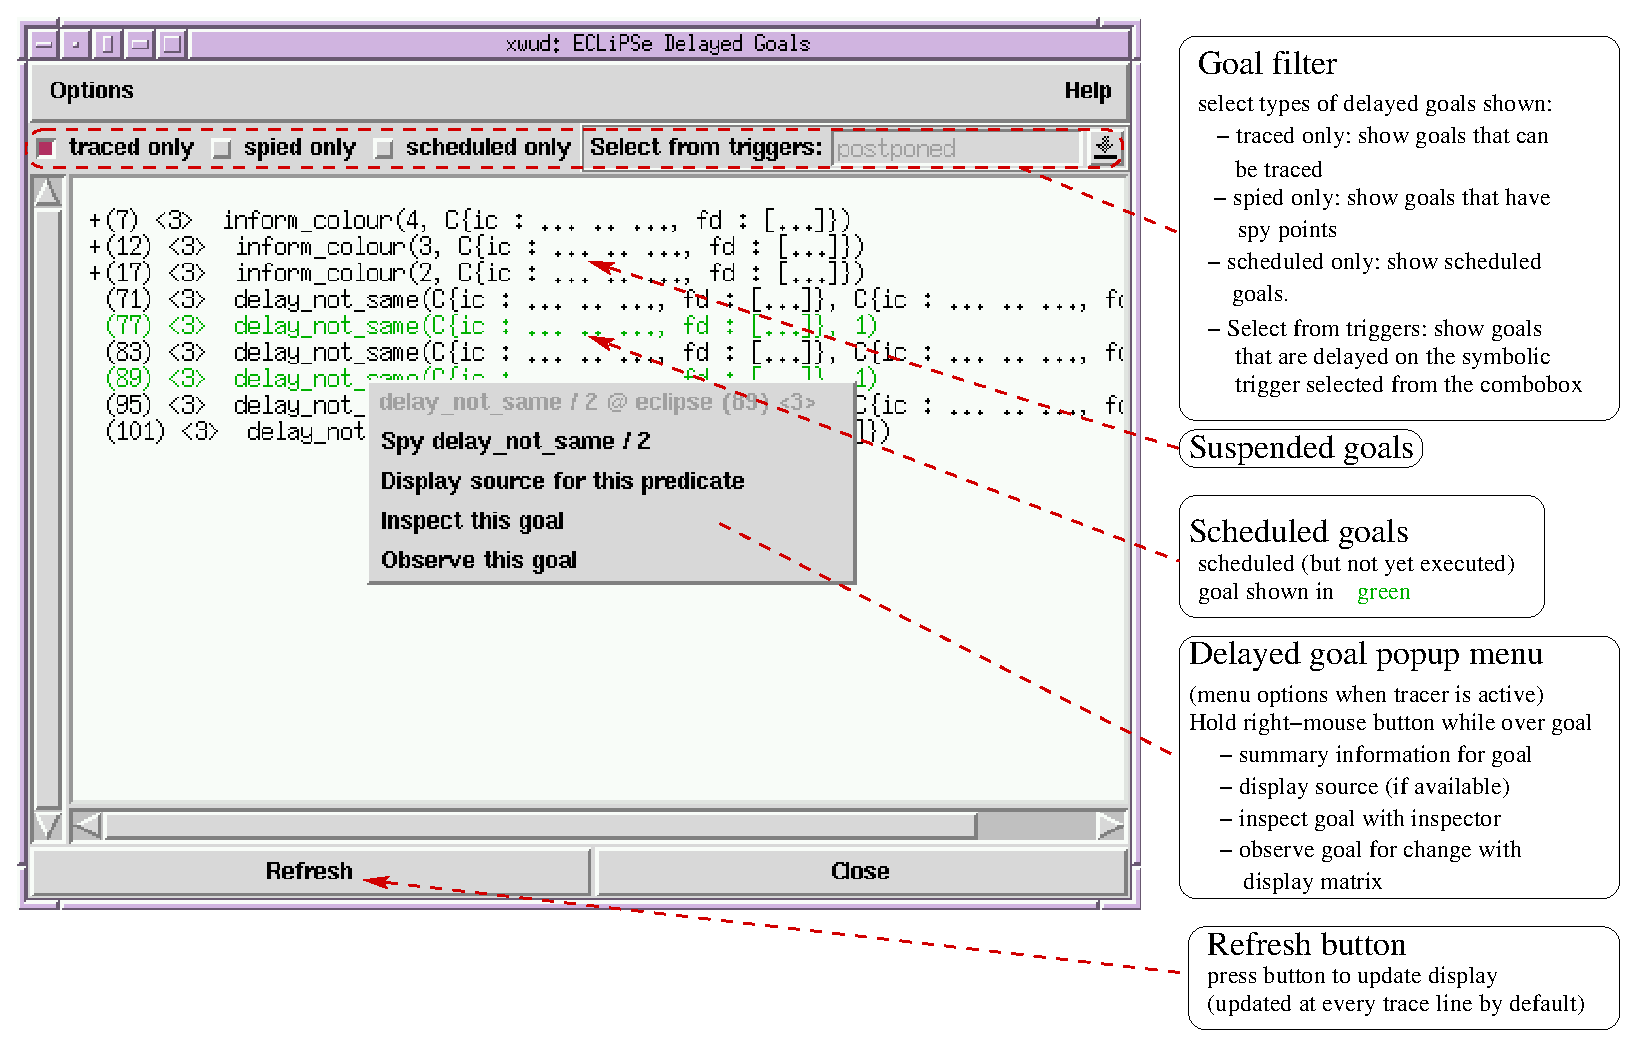
\includegraphics{tkdelayedann.eps}}
\subsection{Tracer}
\index{tracer, development tool}
\resizebox{0.75\textwidth}{!}{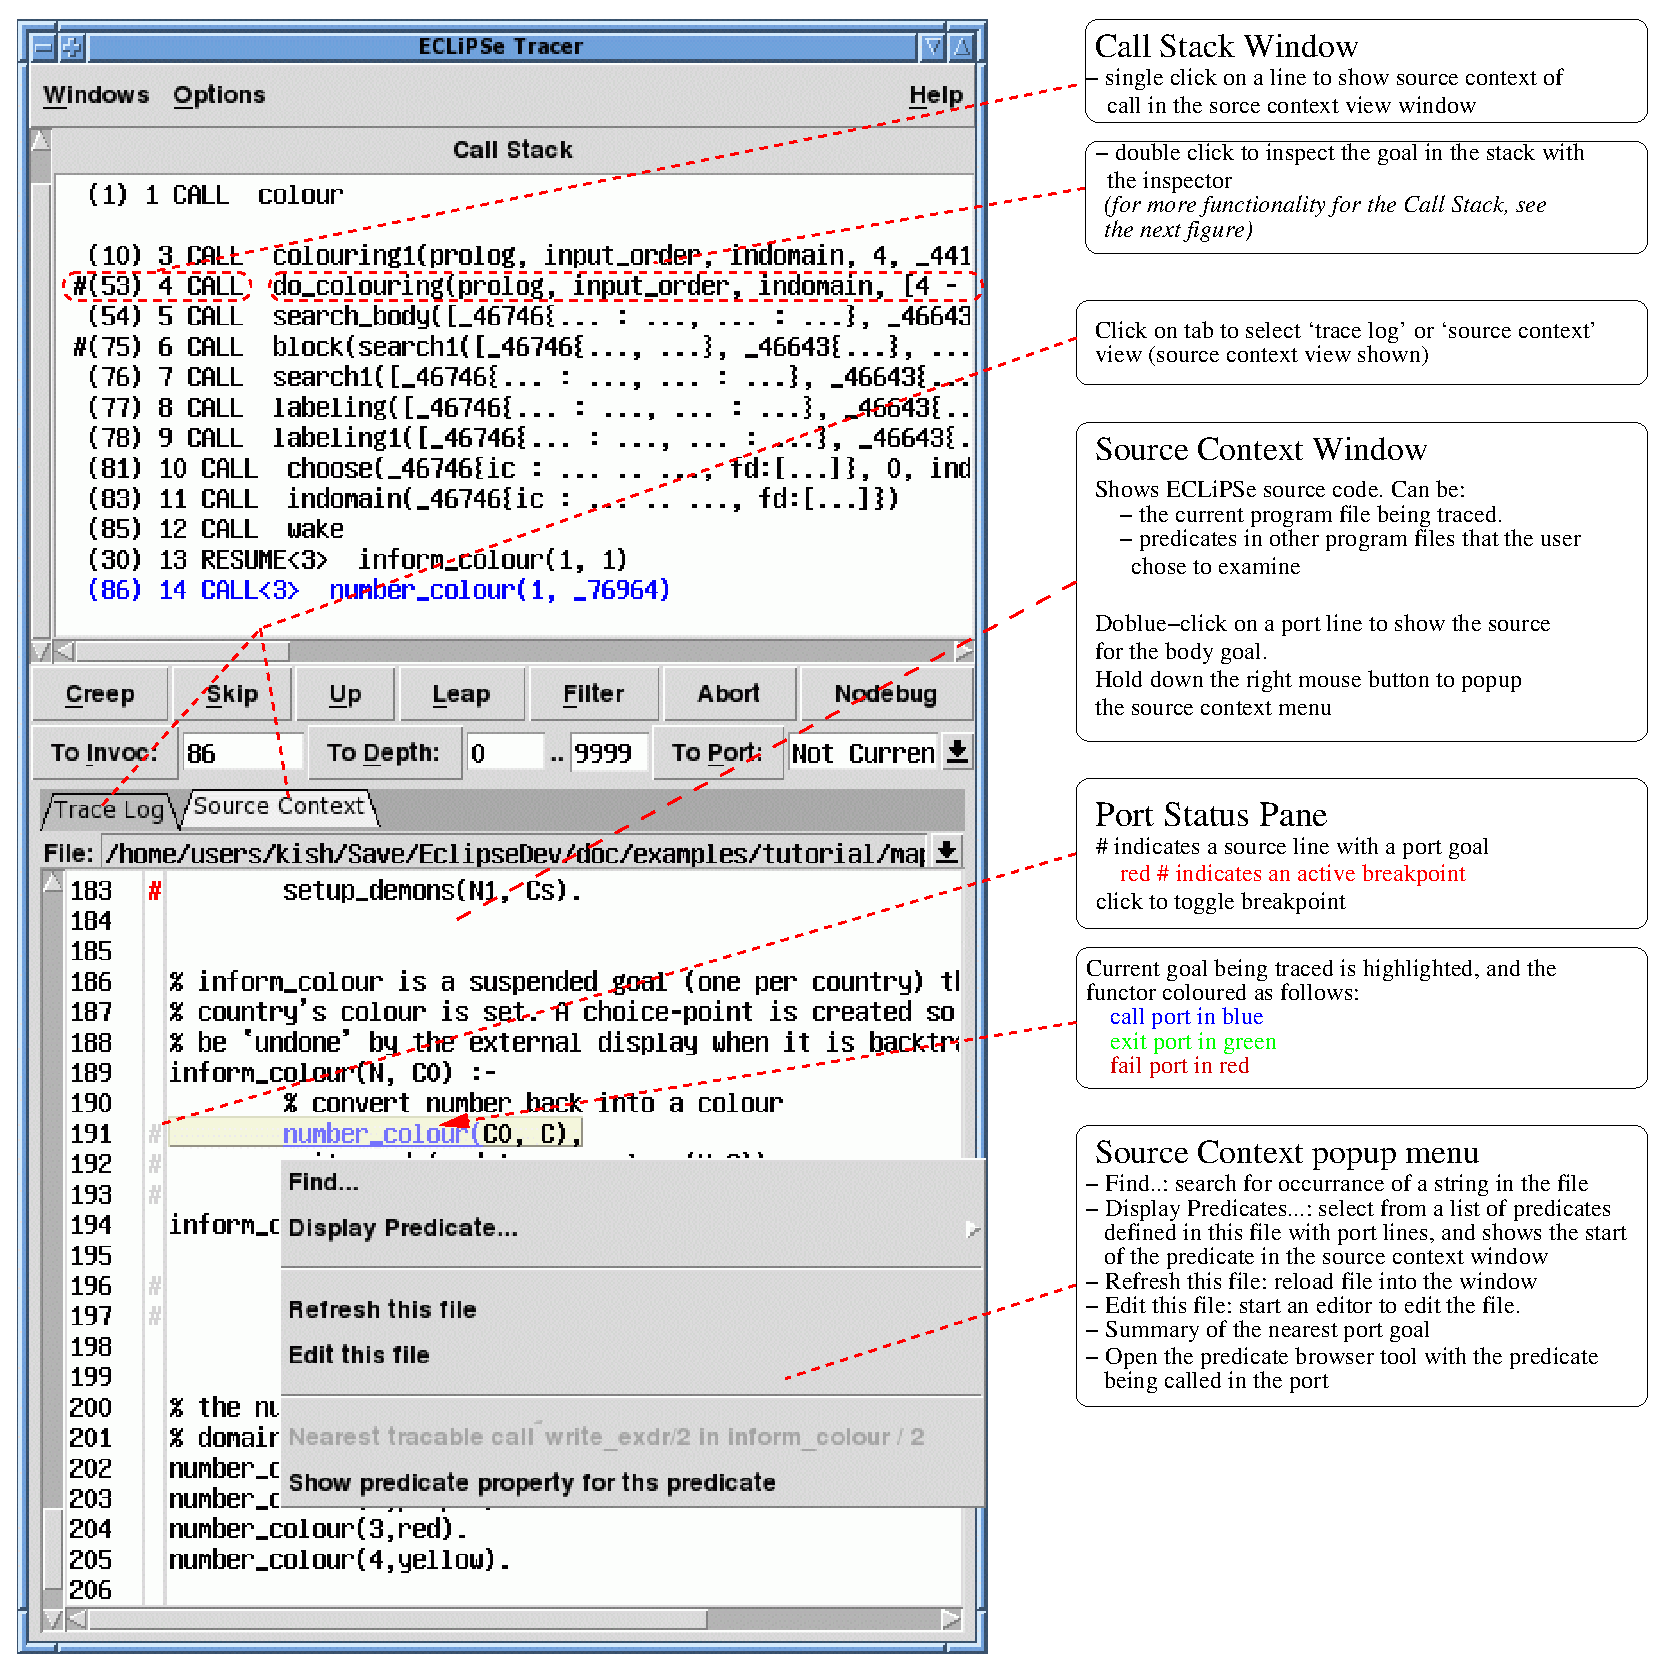
\includegraphics{tktracersourceann.eps}}

\resizebox{0.8\textwidth}{!}{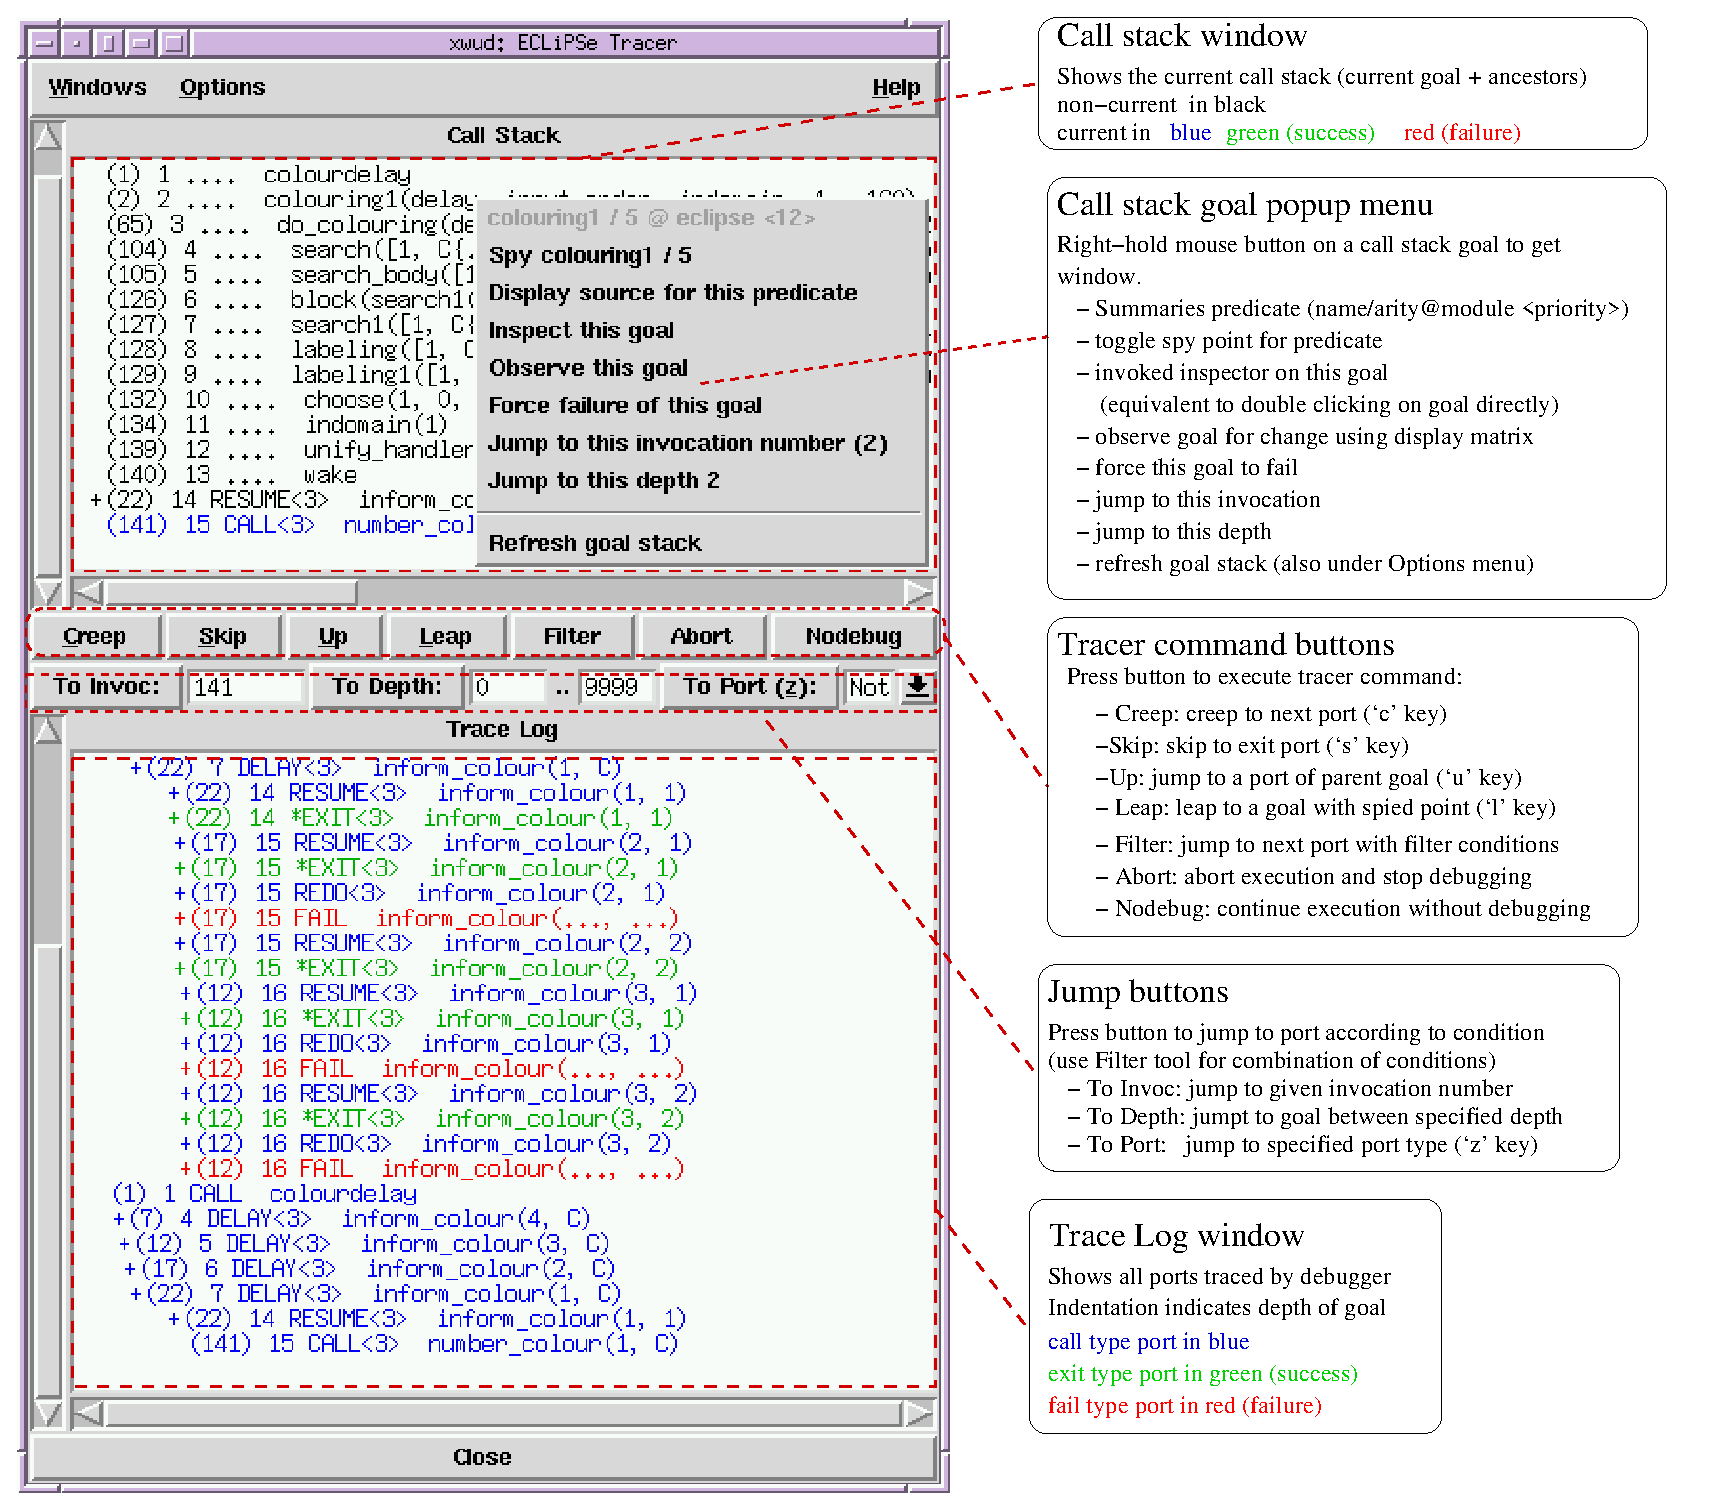
\includegraphics{tktracerann.eps}}

\menu{Options} menu options:
\begin{small}
\begin{description}
\item[Configure filter] Starts the tracer filter window, to allow the
  filter to be configured.
\item[Change print options] Changes the way the tracelines are printed.
\item[Analyse failure] Get the invocation number of the most recent failure
  so that a new run of the  query can jump to its call port.
\item[Refresh goal stack now] Refreshes the Call Stack's display.
\item[Refresh goal stack at every trace line] Select check box to allow the
  call stack to be refreshed automatically every time the tracer stops
\item[Refresh delay goals at every trace line] Select check box to allow
  the Delayed goals viewer to be automatically refreshed every time the
  tracer stops.
\item[Raise tracer window at every tracer line] Select check box to allow
  the tracer window to be raised (uncovered) automatically every time the
  tracer stops.
\end{description}
\end{small}

\subsection{Tracer Filter}
\index{tracer filter, development tool}

\resizebox{0.75\textwidth}{!}{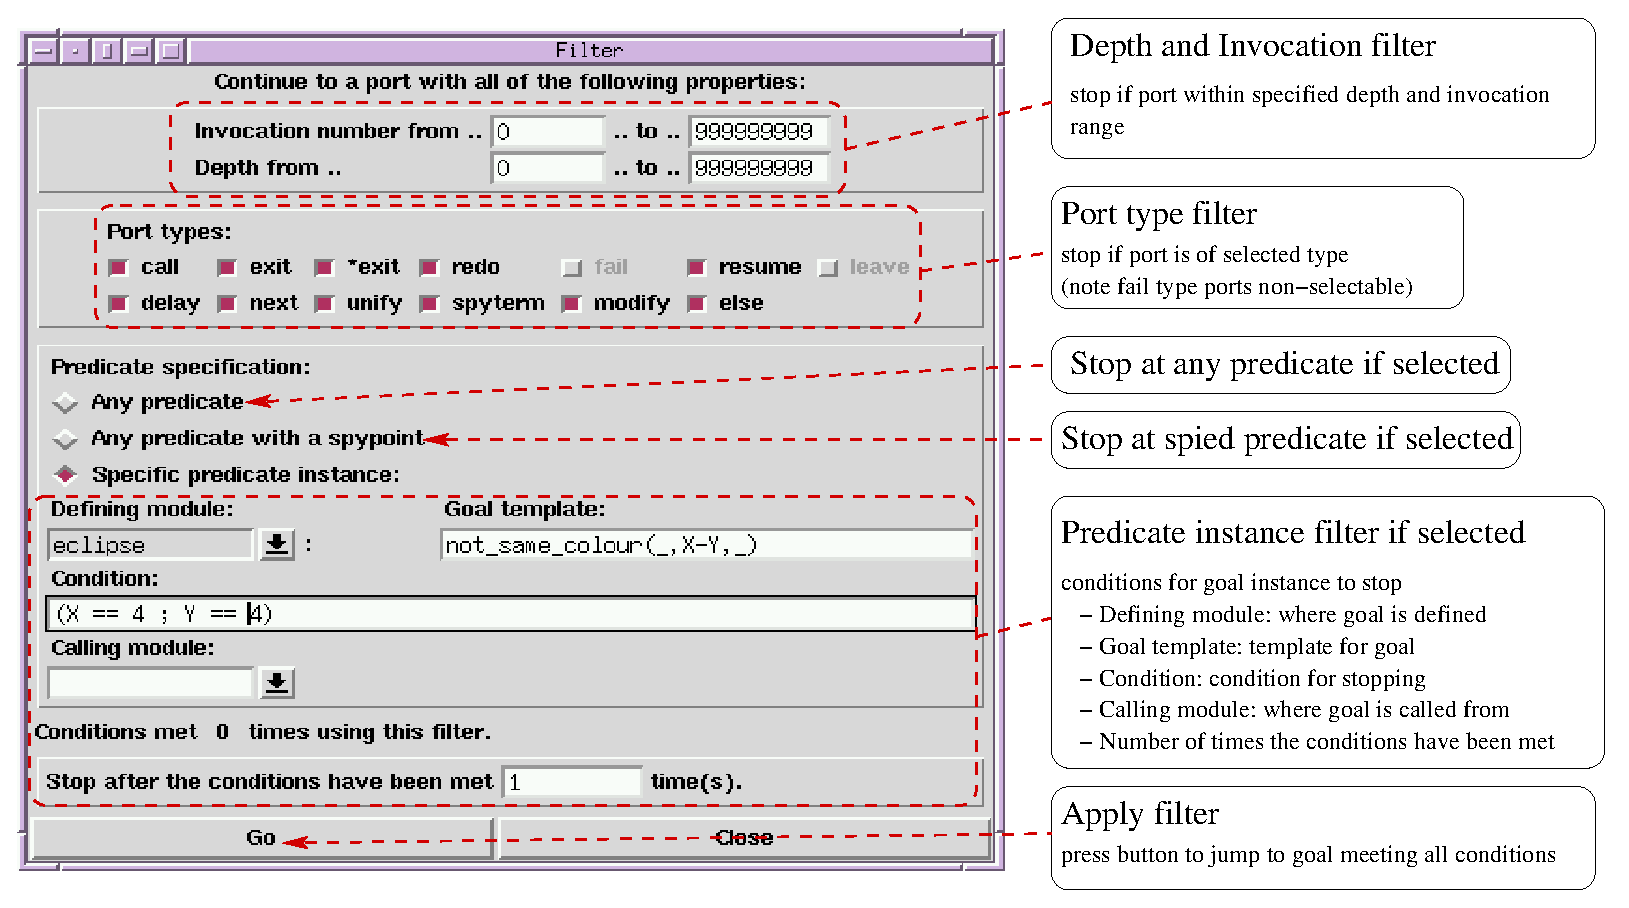
\includegraphics{tkfilterann.eps}}

\subsection{Term Inspector}
\index{term inspector, development tool}

\resizebox{0.8\textwidth}{!}{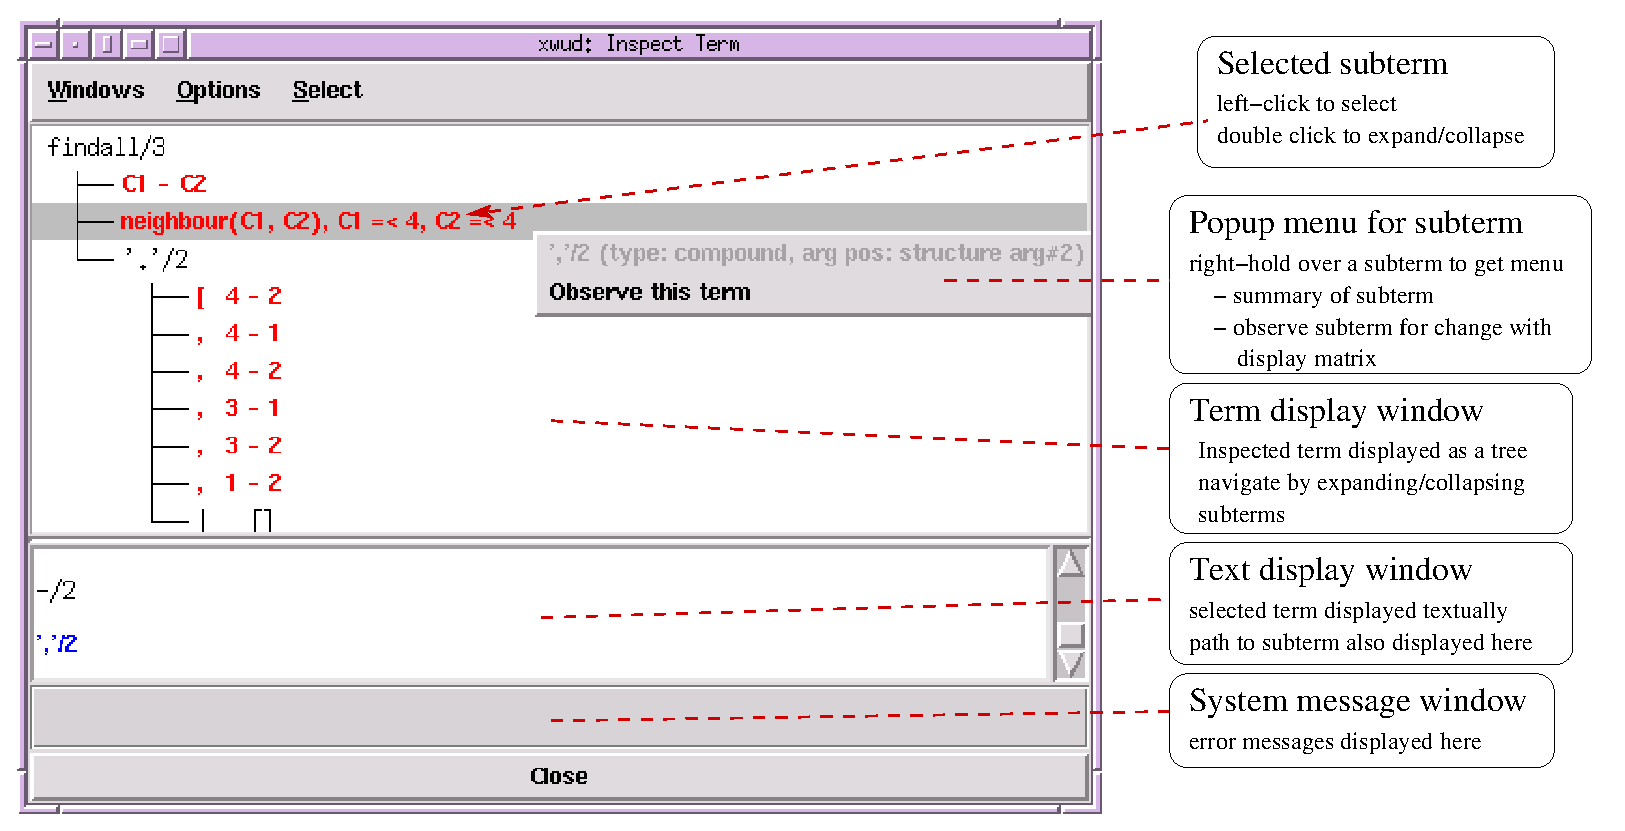
\includegraphics{tkinspectann.eps}}


%HEVEA\cutend
